%% =====================================================================
%% Truthful auctions for last-mile delivery -- Undergraduate thesis, IEM School, International University
%% (VNU-HCM). Format: "IEM-IU Thesis Guidelines (Updated 03/2023)".
%%
%%   * A4, margins top 2.5 / left 3 / right 2 / bottom 2.5 cm, page number
%%     centred 1.5 cm from the bottom edge
%%   * Times New Roman 13 pt body, 14 pt headings, 1.5 line spacing
%%   * Roman page numbers from the Abstract to the List of Symbols,
%%     Arabic numbers from Chapter 1
%%   * Chapters "Chapter n: TITLE" centred at the top; sections 1.1, 1.1.1
%%   * Tables and figures numbered by chapter; table captions above the
%%     table, figure captions below the figure
%%   * APA-style author--year citations, alphabetical reference list
%%
%% Compile with pdfLaTeX (twice, for the table of contents and the cross
%% references). No BibTeX run is needed: the reference list is in
%% references.tex.
%%
%% Source of all numbers: Paper.tex (rev. 2026-09-30), Master_writeup.md
%% (rev. 2, 2026-09-28) and AUDIT_REPORT.md (2026-10-01). Where the audit
%% corrects the paper (label-rule speed-up), the audit is followed.
%% Lines marked "% TODO" need input from the author.
%% =====================================================================
\documentclass[a4paper,12pt,oneside]{report}

% ---------------------------------------------------------------- fonts
\usepackage[T1]{fontenc}
\usepackage{amsmath}
\usepackage{amsthm}               % must be loaded before newtxmath
\usepackage{newtxtext}           % Times New Roman clone
\usepackage{newtxmath}            % matching math fonts (provides \mathbb)
\usepackage[fontsize=13pt]{scrextend}   % 13 pt body text

% ---------------------------------------------------------------- page layout
\usepackage[a4paper,top=2.5cm,bottom=2.5cm,left=3cm,right=2cm,
            footskip=1.0cm]{geometry}   % number sits 1.5 cm above the edge
\usepackage{setspace}
\onehalfspacing

% ---------------------------------------------------------------- packages
\usepackage{booktabs}
\usepackage{array}
\usepackage{multirow}
\usepackage{threeparttable}
\usepackage{graphicx}
\usepackage{float}
\usepackage[chapter]{algorithm}
\usepackage{algpseudocode}
\usepackage{enumitem}
\usepackage{tikz}
\usetikzlibrary{arrows.meta,positioning,fit,backgrounds,shapes.geometric}
\usepackage[labelsep=space,font=normalsize,skip=6pt]{caption}
\usepackage{titlesec}
\usepackage[titles]{tocloft}
\usepackage[round,authoryear]{natbib}
\usepackage[hidelinks]{hyperref}

\graphicspath{{figures/}}

% ---------------------------------------------------------------- headings
% Chapter: "Chapter 1: INTRODUCTION", centred at the top, 14 pt bold,
% followed by a double space.
\titleformat{\chapter}[block]
  {\centering\bfseries\fontsize{14}{18}\selectfont}
  {Chapter \thechapter:}{0.4em}{}
\titlespacing*{\chapter}{0pt}{0pt}{2\baselineskip}
\titleformat{\section}
  {\bfseries\fontsize{13}{16}\selectfont}{\thesection.}{0.5em}{}
\titlespacing*{\section}{0pt}{12pt}{6pt}
\titleformat{\subsection}
  {\bfseries\fontsize{13}{16}\selectfont}{\thesubsection.}{0.5em}{}
\titlespacing*{\subsection}{0.6cm}{10pt}{4pt}
\titleformat{\subsubsection}
  {\bfseries\itshape\fontsize{13}{16}\selectfont}{\thesubsubsection.}{0.5em}{}
\titlespacing*{\subsubsection}{1.2cm}{8pt}{2pt}
\setcounter{secnumdepth}{3}
\setcounter{tocdepth}{2}

% ---------------------------------------------------------------- contents lists
\renewcommand{\cftchappresnum}{Chapter }
\renewcommand{\cftchapaftersnum}{:}
\setlength{\cftchapnumwidth}{5.6em}
\renewcommand{\cftchapfont}{\bfseries}
\renewcommand{\cftchappagefont}{\bfseries}
\renewcommand{\cftchapleader}{\cftdotfill{\cftdotsep}}
\renewcommand{\cftsecaftersnum}{.}
\renewcommand{\cftsubsecaftersnum}{.}
\setlength{\cftsecnumwidth}{2.6em}
\setlength{\cftsubsecnumwidth}{3.4em}
\renewcommand{\cfttoctitlefont}{\hfill\bfseries\fontsize{14}{18}\selectfont}
\renewcommand{\cftaftertoctitle}{\hfill}
\renewcommand{\cftlottitlefont}{\hfill\bfseries\fontsize{14}{18}\selectfont}
\renewcommand{\cftafterlottitle}{\hfill}
\renewcommand{\cftloftitlefont}{\hfill\bfseries\fontsize{14}{18}\selectfont}
\renewcommand{\cftafterloftitle}{\hfill}
\renewcommand{\cfttabpresnum}{Table }
\renewcommand{\cftfigpresnum}{Figure }
\setlength{\cfttabnumwidth}{5.2em}
\setlength{\cftfignumwidth}{5.8em}
\setlength{\cfttabindent}{0pt}
\setlength{\cftfigindent}{0pt}

% ---------------------------------------------------------------- floats
\captionsetup[table]{position=top}
% Ragged-right paragraph column for tables (avoids stretched word spacing)
\newcolumntype{P}[1]{>{\raggedright\arraybackslash}p{#1}}
\floatname{algorithm}{Procedure}
\algrenewcommand\algorithmicrequire{\textbf{Input:}}
\algrenewcommand\algorithmicensure{\textbf{Output:}}
\setlength{\textfloatsep}{14pt plus 2pt minus 4pt}

% ---------------------------------------------------------------- theorems
\newtheorem{theorem}{Theorem}[chapter]
\newtheorem{lemma}[theorem]{Lemma}
\newtheorem{proposition}[theorem]{Proposition}
\newtheorem{corollary}[theorem]{Corollary}
\theoremstyle{definition}
\newtheorem{definition}[theorem]{Definition}
\newtheorem{assumption}{Assumption}
\renewcommand{\theassumption}{A\arabic{assumption}}
\newtheorem{example}[theorem]{Example}
\theoremstyle{remark}
\newtheorem{remark}[theorem]{Remark}

% ---------------------------------------------------------------- notation
\newcommand{\Kstar}{\mathcal{K}^\star}
\newcommand{\lth}{\underline{\theta}}
\newcommand{\uth}{\overline{\theta}}
\newcommand{\R}{\mathbb{R}}
\newcommand{\FD}{\mathrm{FD}}

% ---------------------------------------------------------------- thesis data
\newcommand{\thesistitle}{Truthful Auctions for Last-Mile Delivery with
  Gigworkers and Occasional Drivers}
\newcommand{\THESISTITLE}{TRUTHFUL AUCTIONS FOR LAST-MILE DELIVERY WITH
  GIGWORKERS AND OCCASIONAL DRIVERS}
\newcommand{\studentname}{Tran An Khoa}
\newcommand{\studentid}{IELSIU23040}
\newcommand{\advisorname}{Dr.~Pham Nhat Tan}
\newcommand{\degreename}{Bachelor of Engineering in Logistics and Supply
  Chain Management}
\newcommand{\thesisdate}{December 2026}

% Unnumbered heading that still appears in the table of contents
\newcommand{\frontchapter}[1]{%
  \chapter*{#1}\addcontentsline{toc}{chapter}{#1}}

\begin{document}

% =====================================================================
% Front cover, inside cover and approval page (no page numbers)
% =====================================================================
\pagenumbering{gobble}
%% Front cover (Appendix A of the guideline), inside cover (Appendix B)
%% and approval page (Appendix C). Font sizes follow the Word template:
%% institution lines 14 pt bold, title 22 pt bold, degree line 16 pt,
%% student/advisor 16 pt bold, place and date 14 pt.
%% Cover colour when bound: dark green (bachelor) / blue (master).

\newcommand{\coverpage}{%
\begin{titlepage}
\begin{singlespace}
\centering
{\fontsize{14}{18}\selectfont\bfseries
 VIETNAM NATIONAL UNIVERSITY -- HO CHI MINH CITY\\[2pt]
 INTERNATIONAL UNIVERSITY\\[2pt]
 SCHOOL OF INDUSTRIAL ENGINEERING AND MANAGEMENT\par}
\vspace{1.2cm}

\includegraphics[width=4.2cm]{logoIU.png}\par
\vspace{1.4cm}
{\fontsize{22}{28}\selectfont\bfseries \THESISTITLE\par}
\vspace{1.4cm}
{\fontsize{16}{21}\selectfont Submitted in partial fulfilment of the
 requirements for the Degree of \degreename\par}
\vfill
{\fontsize{16}{22}\selectfont\bfseries
\begin{tabular}{@{}ll@{}}
Student:        & \studentname\\
ID:             & \studentid\\
Thesis Advisor: & \advisorname\\
\end{tabular}\par}
\vspace{1.6cm}
{\fontsize{14}{18}\selectfont Ho Chi Minh City, Vietnam\\ \thesisdate\par}
\end{singlespace}
\end{titlepage}}

% ---------------------------------------------------------------- front cover
\coverpage

% ---------------------------------------------------------------- inside cover
\coverpage

% ---------------------------------------------------------------- approval page
\begin{titlepage}
\begin{singlespace}
\centering
{\fontsize{14}{18}\selectfont\bfseries \THESISTITLE\par}
\vspace{1.2cm}
By\par
\vspace{0.4cm}
{\fontsize{12}{15}\selectfont \studentname\par}
\vspace{1.2cm}
{\fontsize{14}{18}\selectfont Submitted in partial fulfilment of the
 requirements for the Degree of \degreename\par}
\vspace{0.8cm}
{\fontsize{14}{18}\selectfont International University, Ho Chi Minh City\\
 \thesisdate\par}
\vspace{2cm}
\raggedright
{\fontsize{14}{18}\selectfont
Signature of Student: \hrulefill\par
\hfill \studentname\par
\vspace{1.6cm}
Certified by \hrulefill\par
\hfill Thesis Advisor\par
\hfill \advisorname\par
\vspace{1.6cm}
Approved by \hrulefill\par
\hfill Dean of IEM School\par}
\end{singlespace}
\end{titlepage}


% =====================================================================
% Preliminary pages: lowercase Roman numerals
% =====================================================================
\cleardoublepage
\pagenumbering{roman}
\pagestyle{plain}
\frontchapter{Abstract}

Last-mile delivery platforms increasingly buy capacity from a contracted
fixed fleet with a known price, from gigworkers who drive open multi-stop
routes, and from occasional drivers who carry parcels on trips they make
anyway. Crowd drivers' value of time is private, and paying what they claim
invites overstatement. This thesis studies a procurement mechanism in which
truthful reporting is a dominant strategy for both crowd classes: routes are
generated from public data before bidding, winners are selected exactly, and
Vickrey--Clarke--Groves (VCG) payments are paid.

Because the route pool must be fixed before bids are seen, its size is the
bottleneck. A gigworker has no detour budget to bound the search, so her
pool grows as $\Theta(n^B)$ in the number of orders $n$ for a bundle cap $B$,
and only 0.4--1.5\% of generated routes are ever optimal on the test
instances. The thesis asks how far such a pool can be pruned by a rule that
reads neither bids nor other drivers' data.

Routes are generated by a forward label-setting algorithm. An envelope that
completes subset routes with the publicly priced fixed fleet defines a
\emph{local frontier}. The thesis proves that deleting every route outside
it leaves all payments unchanged, because every deleted route has a
substitute that is itself retained. Results planned for the final thesis
concern the minimality and worst-case size of the frontier, a label rule
that prunes during enumeration, and a decomposition of the payment
computation.

The methods were implemented in Python with CPLEX and evaluated in a
pre-registered study on 1,500 synthetic instances with 10 to 20 orders;
route generation was also run on up to 100 orders, and the full evaluation
will be extended to that scale. All solves were optimal and all checks against a brute-force oracle passed. The
frontier removed 75--100\% of the pool without changing any payment, and
where the fixed fleet dominates it certified before bidding that 60\% of the
drivers with a feasible route need not take part. Joint bidding, bundling
and truthful payments mattered only where the crowd competes with the fixed
fleet: there they lowered system cost by 5.8\% and 11.3\% and carried a
14.1\% payout premium (medians). The fixed-fleet price decides which regime
applies. Future work should study rules that use other drivers' public data
and richer driver reports.

\medskip
\noindent\textbf{Keywords:} Crowdshipping; Mechanism design; VCG auction;
Pickup and delivery; Column pruning

\frontchapter{Acknowledgements}

First and foremost, I would like to express my deepest gratitude to my
thesis advisor, \advisorname, for the guidance, patience and encouragement
I received throughout this thesis. The advisor's questions pushed me to
state every claim precisely, to check every result against an independent
test, and to be honest about what the results do not show. This thesis
would not have reached its present form without that support.

I am grateful to the lecturers of the School of Industrial Engineering and
Management, International University -- Vietnam National University Ho Chi
Minh City, whose courses in operations research, optimisation and logistics
gave me the foundation on which this work is built. I also thank the
members of the thesis committee and the reviewers for the time they devote
to reading and evaluating this thesis.

My thanks also go to my friends and classmates for the discussions,
feedback and company during the years of study.

Finally, I owe my greatest debt to my family, whose love, patience and
constant support made my studies possible. This thesis is dedicated to them.

\vspace{1cm}
\noindent Ho Chi Minh City, \thesisdate\par
\noindent \studentname


\clearpage
\phantomsection
\addcontentsline{toc}{chapter}{Table of Contents}
\renewcommand{\contentsname}{Table of Contents}
\tableofcontents

\clearpage
\phantomsection
\addcontentsline{toc}{chapter}{List of Tables}
\listoftables

\clearpage
\phantomsection
\addcontentsline{toc}{chapter}{List of Figures}
\listoffigures

\clearpage
\frontchapter{List of Abbreviations}

\begin{singlespace}
\begin{tabular}{@{}P{3.2cm}P{11.5cm}@{}}
DSIC     & Dominant-strategy incentive compatibility\\[3pt]
ESPPRC   & Elementary shortest path problem with resource constraints\\[3pt]
FD       & Fixed-capacity (contracted) fleet, the non-strategic outside option\\[3pt]
GW       & Gigworker, a crowd driver who drives an open route\\[3pt]
HEUR     & Heuristic route menu built from a fixed, bid-independent partition of the orders\\[3pt]
IC       & Incentive compatibility\\[3pt]
IQR      & Interquartile range\\[3pt]
IR       & Individual rationality\\[3pt]
LP       & Linear programming\\[3pt]
MILP     & Mixed-integer linear programming\\[3pt]
OD       & Occasional driver, a crowd driver who detours from a personal trip\\[3pt]
PAB      & Pay-as-bid (first-price) mechanism\\[3pt]
PAB-BR   & Pay-as-bid with unilateral best-response reports\\[3pt]
PDP(TW)  & Pickup and delivery problem (with time windows)\\[3pt]
POSTED   & Posted-price mechanism\\[3pt]
RQ       & Research question\\[3pt]
TW       & Time window\\[3pt]
VCG      & Vickrey--Clarke--Groves (mechanism or payment)\\[3pt]
VRP      & Vehicle routing problem\\[3pt]
VRPOD    & Vehicle routing problem with occasional drivers\\[3pt]
WDP      & Winner-determination problem\\
\end{tabular}
\end{singlespace}

\clearpage
\frontchapter{List of Symbols}

\begin{singlespace}
\small
\renewcommand{\arraystretch}{1.0}
\begin{tabular}{@{}P{2.6cm}P{12.1cm}@{}}
\multicolumn{2}{@{}l}{\textbf{Sets and indices}}\\[2pt]
$O$, $o$ & Set of orders, an order\\
$N=G\cup C$ & Set of strategic drivers: gigworkers $G$ and occasional drivers $C$\\
$i,j,k$ & Drivers\\
$R_i$ & Route pool of driver $i$, fixed before reports are collected\\
$r$, $0_i$ & A route; the empty (idle) route of driver $i$\\
$S_r$ & Bundle (set of orders) served by route $r$\\
$D(r)$ & Subset routes of $r$: routes $r'$ of the same driver with $S_{r'}\subseteq S_r$\\
$\Kstar_i$ & Local pruning frontier of driver $i$\\
$\mathcal G$, $\mathcal P$ & Conflict graph between drivers; its connected components\\[3pt]
\multicolumn{2}{@{}l}{\textbf{Parameters}}\\[2pt]
$p_o$, $d_o$ & Pickup and delivery node of order $o$\\
$q_o$, $q(A)$ & Public fixed-fleet price of order $o$; $q(A)=\sum_{o\in A}q_o$\\
$B$ & Bundle cap (maximum number of orders per route)\\
$d(\cdot,\cdot)$, $\tau(\cdot,\cdot)$ & Travel distance (km) and travel time (min)\\
$e_v$, $l_v$, $s_v$ & Opening time, closing time and service time of stop $v$\\
$t_0$ & Departure time of a driver\\
$\tau_i$ & Detour budget of occasional driver $i$ (min)\\
$\kappa_i$ & Distance-cost coefficient of driver $i$ (cost units per km)\\
$K_{ir}$, $W_{ir}$ & Distance cost (cost units) and working time (h) of route $r$ of driver $i$\\
$\Theta=[\lth,\uth]$ & Report domain announced before bidding\\[3pt]
\multicolumn{2}{@{}l}{\textbf{Private information, reports and decisions}}\\[2pt]
$\theta_i$ & Private value of time of driver $i$ (cost units per hour)\\
$b_i$ & Report (bid) of driver $i$\\
$C_{ir}(\theta_i)$ & True cost of route $r$ for driver $i$: $K_{ir}+\theta_iW_{ir}$\\
$c_{ir}(b_i)$ & Reported cost: $K_{ir}+b_iW_{ir}$\\
$x_{ir}$ & 1 if driver $i$ receives route $r$, 0 otherwise\\
$z_o$ & 1 if order $o$ is delegated to the fixed fleet, 0 otherwise\\[3pt]
\multicolumn{2}{@{}l}{\textbf{Values and derived quantities}}\\[2pt]
$V(R;b)$ & Optimal value of the winner-determination problem on pools $R$ at reports $b$\\
$V_{-k}(R;b)$ & Optimal value with driver $k$ removed\\
$p_i$ & VCG (Clarke-pivot) payment to driver $i$\\
$E_r(b)$ & FD-completion envelope of route $r$\\
$\mu_r(b)$ & Local margin of route $r$: $E_r(b)-c_r(b)$\\
$\Pi$, $\Pi^\star$ & A local pruning rule; the frontier rule\\
$\Delta D$, $\delta$, $A$, $\beta$ & Distance saving, time saving, absorption term and lower bound of the label rule\\
$Z^\ast(S;A)$ & Optimal value restricted to drivers $S$ and orders $A$\\
\end{tabular}
\end{singlespace}


% =====================================================================
% Main text: Arabic numerals
% =====================================================================
\clearpage
\pagenumbering{arabic}
% =====================================================================
\chapter{INTRODUCTION}
\label{ch:intro}
% =====================================================================

\section{Background}
\label{sec:background}

The last mile, the final leg from a pickup point to the customer, is widely
regarded as the most expensive and least efficient part of a parcel's
journey, and it has attracted a large body of operational research on new
delivery concepts \citep{boysen2021lastmile}. One of the most visible of
these concepts is \emph{crowdsourced delivery} (also called crowdshipping):
instead of relying only on employed drivers, a platform hands orders to
independent individuals who are paid per task. Reviews of the field document
both the rapid growth of such platforms and the new planning problems they
create, because the people who deliver are not employees and their capacity
and costs are not under the platform's control
\citep{alnaggar2021crowdsourced,savelsbergh2022challenges,savelsbergh2024update}.
Crowdshipping is also studied as a lever for more sustainable urban
logistics, since parcels can ride along on trips that take place anyway
\citep{mohri2023crowdshipping}.

In practice a delivery platform therefore combines three sources of
capacity \citep{archetti2016vrpod,luy2024workforce}, summarised in
Table~\ref{tab:classes}:
\begin{itemize}[leftmargin=*,itemsep=2pt]
\item a \emph{fixed-capacity fleet} (FD) operated under contract, which
serves any order at a known, published price;
\item \emph{gigworkers} (GW), who accept multi-stop routes through an
application. A gigworker starts from her current location, and her route is
\emph{open}: it ends at the last delivery;
\item \emph{occasional drivers} (OD), who carry parcels along a personal
trip they would make anyway. Their route must end at their own destination,
and the extra time they are willing to spend is limited by a \emph{detour
budget}.
\end{itemize}

\begin{table}[t]
\centering
\caption{The three sources of last-mile capacity considered in this thesis}
\label{tab:classes}
\small
\begin{tabular}{P{2.5cm}P{4.3cm}P{2.0cm}P{5.0cm}}
\toprule
Class & Route geometry & Strategic? & Private information\\
\midrule
Gigworker (GW) & Open route from the current location, ends at the last delivery & Yes & Value of time $\theta_i$ (one scalar)\\
Occasional driver (OD) & From origin to personal destination, limited by a detour budget & Yes & Value of time $\theta_i$ (one scalar)\\
Fixed fleet (FD) & Not routed in the model; serves any order & No & None: public price $q_o$ per order\\
\bottomrule
\end{tabular}
\par\smallskip\footnotesize Source: taxonomy adopted from \citet{luy2024workforce}.
\end{table}

The fixed fleet has a known price. The other two sources do not. How much
an hour of driving is worth to a particular driver --- her \emph{value of
time} --- is private information, and it determines her cost of serving a
route. A platform that pays drivers what they claim invites them to
overstate it. The classical remedy from mechanism design is the
Vickrey--Clarke--Groves (VCG) mechanism: the platform selects the
allocation that minimises total reported cost and pays each winner her
externality on the others. Under this payment rule, reporting the true cost
is a dominant strategy, that is, the best action for a driver regardless of
what the others report \citep{nisan2007agt}. In routing applications the
mechanism is implemented in four steps \citep{zou2022mechanisms,li2026auction}:
the platform generates candidate routes, collects one scalar bid per driver,
solves a set-partitioning winner-determination problem (WDP), and re-solves
it once per winner to compute the Clarke-pivot payments.

This thesis studies such a procurement mechanism for a platform that buys
from \emph{both} crowd classes at once, with the fixed fleet as a publicly
priced outside option. Studying the two crowd classes together matters because their capacities
are complementary: an occasional driver is cheap but only for orders that
lie along her trip, whereas a gigworker can go anywhere but charges for all
of her working time.

\section{Problem Statement}
\label{sec:problem}

\subsection{The need for a bid-independent route pool}

For the VCG mechanism above to remain truthful, the set of routes among
which the platform chooses must be fixed \emph{before} any bid is seen. The
mechanism is then VCG on a bid-independent range, and dominant-strategy
incentive compatibility follows from the maximal-in-range argument of
\citet{nisan2007computationally}. If the platform let the bids influence
which routes are generated --- for example by generating routes with column
generation, whose pricing step depends on dual values and hence on the bids
--- a driver could change the set of available routes by changing her bid,
and truthfulness would no longer be guaranteed.

\subsection{The pool is the bottleneck, and the two classes differ}

The price of this requirement is the size of the route pool. For an
occasional driver, the detour budget anchors the search: adding orders to a
bundle can only lengthen the detour, so a bundle whose detour already
exceeds the budget can be discarded together with all its supersets before
any visiting sequence is enumerated \citep{li2026auction}. A gigworker has no
such anchor. Her route is open and is limited only by time windows. Two
orders may each be servable on their own while the pair is not, and a bundle
of distant orders remains feasible whenever the windows are wide. Her pool
therefore grows as $\Theta(n^B)$ in the number of orders $n$ for a bundle cap
$B$. On the experimental instances of this thesis, the pool of an occasional
driver is only 0.7--1.7\% of that of a gigworker, and on five instances only
0.4--1.5\% of all generated routes are optimal for \emph{any} of 1,000 sampled
bid profiles. Most of the pool is never used, yet the platform cannot tell
in advance which part.

Removing routes is not straightforward either. Every cheap reduction rule
that was tried during the development of this thesis either deleted routes
that some bid profile needs, or pruned almost nothing
(Section~\ref{sec:selection} lists them). Two obstacles explain why:
\begin{enumerate}[leftmargin=*,itemsep=2pt]
\item any rule that reads the bids changes the allocation range and can
destroy truthfulness;
\item any rule that reasons about \emph{other} drivers must, in the worst
case, solve the winner-determination problem itself, which is NP-hard
(Remark~\ref{rem:scope}).
\end{enumerate}
What remains are \emph{local, bid-independent} rules, which look only at
the pruned driver's own data and the public prices. No study in the
literature characterises how far such rules can go
(Chapter~\ref{ch:related}).

\subsection{Research questions}

The problem leads to one central question and four technical
sub-questions. This proposal answers TQ1 in Chapter~\ref{ch:solution};
TQ2--TQ4 are planned for the final thesis (Section~\ref{sec:sd-planned}).

\begin{quote}
\emph{How far can a route pool be pruned, before bids are observed, by a rule
that uses only the pruned driver's own data, without changing the outcome of
the VCG mechanism?}
\end{quote}

\begin{description}[leftmargin=1.2cm,style=nextline,itemsep=2pt]
\item[TQ1] Which routes can a local bid-independent rule safely delete, and
is there a smallest pool that every such rule must keep?
\item[TQ2] How large can that smallest pool be, and does it contain routes
that are never useful?
\item[TQ3] Can the pruning be moved inside the route enumeration so that
fewer partial routes are explored, without losing safety?
\item[TQ4] Can the repeated counterfactual solves required by the payments be
decomposed into smaller problems, and when does this fail?
\end{description}

Since the mechanism is meant to be used by a platform, the thesis also asks
five empirical questions about its economic and computational behaviour,
which are answered by the computational study (Chapter~5):

\begin{description}[leftmargin=1.2cm,style=nextline,itemsep=2pt]
\item[RQ1] Does letting gigworkers and occasional drivers bid jointly lower
system cost compared with using either class alone or consulting them in
sequence?
\item[RQ2] Does endogenous bundling --- letting the market choose among
platform-generated bundles --- add value compared with single-order routes
and with a fixed bundling heuristic?
\item[RQ3] What does truthful procurement cost compared with a
full-information benchmark, pay-as-bid and posted prices?
\item[RQ4] How much of the pool does the frontier remove, does it change any
payment, and what does it save in computation?
\item[RQ5] Are the conclusions robust to time windows, detour budgets,
fixed-fleet prices, spatial clustering, type dispersion and instance size?
\end{description}

\section{Objectives of the Study}
\label{sec:objectives}

\subsection{General and specific objectives}

The general objective is to design, analyse and evaluate a truthful
procurement mechanism in which gigworkers and occasional drivers bid jointly
for platform-generated route bundles, with the fixed fleet as a publicly
priced outside option, and to characterise exactly how far its route pool
can be reduced without affecting the mechanism. The specific objectives are:
\begin{enumerate}[label=O\arabic*.,leftmargin=1.2cm,itemsep=2pt]
\item To formulate the procurement problem of a static dispatch session as a
mechanism: a cost model for the two crowd classes, a winner-determination
model, and Clarke-pivot payments.
\item To develop a complete, bid-independent route-generation algorithm for
both driver classes (Algorithm~A).
\item To define a local pruning rule (the local frontier), prove that it is
safe (TQ1), and determine whether it is minimal and how large it can be
(TQ2).
\item To develop and prove a label rule that applies the frontier reasoning
during route generation (TQ3), and to establish when payment counterfactuals
decompose (TQ4).
\item To implement the complete pipeline and verify every component against
an independent brute-force oracle.
\item To evaluate the mechanism in a pre-registered computational study
(RQ1--RQ5).
\end{enumerate}

\subsection{Beneficiaries and expected outputs}

The results address three groups.
\emph{Delivery platforms} obtain a procurement procedure that remains
correct when the crowd becomes competitive, and a certificate, computed
before any bid is collected, that tells them whether an auction is worth
opening and which drivers need to be invited. \emph{Drivers} benefit
because truthful reporting is their best strategy, so they need no
strategic reasoning, and because a winner is never paid less than her
reported cost. \emph{Researchers} in routing and mechanism design obtain a
provably safe way to reduce route pools before bidding, which applies to any
set-partitioning auction with a priced outside option.

The expected outputs are:
\begin{itemize}[leftmargin=*,itemsep=2pt]
\item a three-stage procurement pipeline (route generation, winner
determination, payments) with a provably safe pruning step in between;
\item a theorem, with full proof, that pruning the pool to the local frontier
is safe, followed in the final thesis by results on its minimality and
worst-case size, the label rule and payment decomposition;
\item a tested implementation in Python with the CPLEX solver, a synthetic
instance generator and locked, hashed experiment parameters;
\item a computational study that quantifies when joint bidding, bundling and
truthful payments matter.
\end{itemize}

\subsection{Expected scientific contributions}

\begin{enumerate}[leftmargin=*,itemsep=3pt]
\item \emph{The local pruning frontier} (Theorem~\ref{thm:frontier}, proved
in this proposal). An envelope compares each route with the cheapest subset
route of the same driver whose unserved orders are sent to the fixed fleet,
uniformly over the admissible report range. Deleting every route outside the
resulting frontier preserves the optimal value of the winner-determination
problem, every counterfactual value and therefore all VCG payments, because
every deleted route has a substitute that is itself retained.
\item \emph{Minimality and the price of locality} (planned). Every route in
the frontier should be indispensable in some instance that looks the same
from the driver's own data, and a single gigworker's frontier can contain
$\Theta(n^B)$ routes that are never optimal.
\item \emph{A safe label rule} (planned). Rollback pruning
\citep{lozano2016exact} cannot be transferred directly, because working time
is priced and waiting is allowed; a correction for waiting makes it safe.
\item \emph{Payment decomposition with a matching negative result}
(planned). With a separable outside option the counterfactual solves
decompose along the components of a conflict graph; a shared capacity on the
outside option breaks the decomposition.
\item \emph{A pre-registered computational study} of RQ1--RQ5, in which all
parameters were locked and hashed before the main runs.
\end{enumerate}

Two things are \emph{not} claimed. The incentive property is not new: the
mechanism is exact VCG on a bid-independent range, and its truthfulness is
classical. Nor is the three-class driver taxonomy, which is adopted from
\citet{luy2024workforce}.

\subsection{Design requirements}

The mechanism and its implementation must satisfy the requirements in
Table~\ref{tab:requirements}. Requirements R1--R7 are correctness
requirements that the design must meet exactly; R8 and R9 are practical
requirements.

\begin{table}[t]
\centering
\caption{Design requirements of the procurement system}
\label{tab:requirements}
\small
\begin{tabular}{P{0.8cm}P{3.6cm}P{9.6cm}}
\toprule
No. & Requirement & Description\\
\midrule
R1 & Truthfulness (DSIC) & Reporting the true value of time is a dominant strategy for every driver of both classes.\\
R2 & Individual rationality & A winner is paid at least her reported cost; a loser pays and receives nothing.\\
R3 & Service coverage & Every order is served exactly once, by one selected route or by the fixed fleet.\\
R4 & Exactness & Every winner-determination and counterfactual problem is solved to proven optimality (zero gap).\\
R5 & Bid independence & No step before report collection reads a report; the pool is fixed and hashed before bidding.\\
R6 & Deterministic tie-breaking & Ties among optimal solutions are broken by a rule that does not depend on reports.\\
R7 & Safe pruning & Any pool reduction leaves the optimal value, every counterfactual value and every payment unchanged for every admissible report profile.\\
R8 & Tractability & The complete pipeline finishes within 300 seconds per instance up to 30 orders on a single CPU thread, and route generation remains tractable for instances of 100 orders or more.\\
R9 & Reproducibility & Parameters are fixed and hashed before the main runs; every component is checked against an independent oracle.\\
\bottomrule
\end{tabular}
\end{table}

\section{Scope and Limitation}
\label{sec:scope}

\subsection{Scope}

\paragraph{Problem setting.} The study considers a single, static and
deterministic dispatch session: all orders and drivers are known when the
session opens, travel times are deterministic, and the mechanism is run once.
Every order must be served (mandatory fulfilment), each driver receives at
most one route (unit demand), and routes carry at most $B$ orders. Each
driver has one private parameter, her value of time; all other driver data
are public or committed before the session opens.

\paragraph{Instances and data.} All experimental instances are synthetic.
They are produced by an instance generator on a plane with dispersed pickups
and deliveries, time windows of 120 minutes, a detour budget of 30 minutes
for occasional drivers, 5 minutes of service per stop and a speed of
20\,km/h. The distance coefficient is $\kappa=1$ cost unit per kilometre,
values of time are drawn from $U[18,25]$ cost units per hour for both
classes, and the fixed-fleet price of order $o$ is
$q_o=8+3\max\{0,\mathrm{dist}_o-1\}$, where $\mathrm{dist}_o$ is its
pickup--delivery distance in kilometres. The main grid crosses five levels of
an \emph{alignment} parameter (how strongly occasional drivers' trips overlap
the demand region), three instance sizes $n\in\{10,15,20\}$ and four supply
mixes with two or three drivers of each class, with 25 replications per
cell (1,500 instances). Robustness tests extend the size to $n=30$. The
bundle cap is $B=3$, with $B=4$ as a sensitivity case for $n\le 15$, and the
report domain is $\Theta=[18,25]$. No time frame of data collection applies,
since no field data are used.

\paragraph{Instance size.} Small instances are not the limit of the method.
A separate scaling study has already run the route-generation algorithm
(Algorithm~A) on instances of the same generator with up to $n=100$ orders,
bundle caps $B\in\{2,3,4\}$ and time windows of 30 to 240 minutes
(Section~\ref{sec:sd-algA}). The results chapter will extend the evaluation of
the complete mechanism to large instances with $n\in\{50,75,100\}$ orders,
and to larger instances where the time budget allows, so that its
behaviour at the scale of a real dispatch session can be assessed.

\paragraph{Tools.} The pipeline is implemented in Python~3.7.7. The
winner-determination and counterfactual problems are solved with
IBM ILOG CPLEX~12.10 on one thread with zero relative and absolute gap
tolerances.

\subsection{Main assumptions}

\begin{enumerate}[label=(\roman*),leftmargin=1cm,itemsep=2pt]
\item Static, deterministic, single-session procurement.
\item Mandatory fulfilment: each order is served exactly once, by a route or
by the fixed fleet.
\item The fixed fleet is uncapacitated and serves each order at a public,
fixed price $q_o$.
\item Unit demand: each driver receives at most one route.
\item The allocation range (bundle cap $B$, route generation and any
pruning) is fixed before bids.
\item Single-parameter private information: a driver's cost is affine in
her value of time, $C_{ir}=K_{ir}+\theta_iW_{ir}$
(Section~\ref{sec:sd-costs} explains why this is an empirical approximation
rather than a mere convenience).
\item Occasional drivers' destinations and detour budgets are public, or are
committed before the session opens.
\item Travel distances and times satisfy the triangle inequality; arriving
before a time window opens is met by waiting.
\end{enumerate}

\subsection{Limitations}

\begin{itemize}[leftmargin=*,itemsep=2pt]
\item \emph{Synthetic data.} All instances are synthetic and static; no
field data from a delivery platform were available. The fixed-fleet price
was calibrated on a pilot without corridor concentration, and that
calibration did not carry over to the main grid, so the alignment levels do
not order the regimes monotonically by how competitive the crowd is. Results
are therefore reported by regime and observed fixed-fleet share.
\item \emph{Information structure.} Treating occasional drivers' destination
and detour budget as public is a restriction: \citet{li2026auction} let
carriers report four parameters. Private costs are single-parameter and
affine in the report.
\item \emph{Report domain.} Pruning requires a report domain announced in
advance. The pay-as-bid benchmark inherits that bound, which favours it.
\item \emph{Scale.} The economic experiments completed so far cover
$n\le 30$; at $n=100$ only route generation has been measured so far. The
largest bundle cap ($B=4$) was not evaluated at $n=20$, and the scaling study
shows that it becomes intractable before $n=50$, so large instances are
limited to $B\le 3$. The robustness experiment is centred on the least
competitive regime.
\item \emph{Implementation.} The label rule has been integrated only into an
experimental build of the route generator, and in pure Python its extra
bookkeeping currently makes route generation slower
(Section~\ref{sec:sd-label}). The payment decomposition requires a
separable outside option.
\item \emph{Out of scope.} The study makes no claims about online arrivals,
stochastic travel times, budget balance, collusion, false-name bids or
fairness.
\end{itemize}

\section{Structure of the Thesis}

Chapter~\ref{ch:related} introduces the theoretical foundations and reviews
the literature on crowdshipping, procurement mechanisms, column pool
reduction, label dominance and VCG payment computation, and describes the
candidate solution methods. Chapter~\ref{ch:method} compares these
candidates, selects the approach and presents the design of the proposed
system. Chapter~\ref{ch:solution} develops the solution: the mathematical
model, the route-generation algorithm, the local pruning frontier and its
safety theorem, payment computation, the results planned for the final
thesis, a complete numerical example, the implementation and a comparison of
alternatives. The computational study (Chapter~5) and the conclusions
(Chapter~6) follow. The proof of the key lemma is in
Appendix~\ref{app:proofs}.

% =====================================================================
\chapter{RELATED WORKS}
\label{ch:related}
% =====================================================================

This chapter first introduces the theoretical foundations on which the
thesis builds (Section~\ref{sec:overview-foundations}): crowdsourced
last-mile delivery, pickup-and-delivery routing, mechanism design, and
column reduction. Section~\ref{sec:litreview} reviews five streams of
literature, classifies them and positions the thesis against the closest
studies. Section~\ref{sec:candidates} describes the candidate methods for
each component of the system, which Chapter~\ref{ch:method} compares.

\section{Overview}
\label{sec:overview-foundations}

\subsection{Crowdsourced last-mile delivery}

\citet{archetti2016vrpod} introduced the \emph{vehicle routing problem with
occasional drivers} (VRPOD): a company that operates its own fleet may also
use ordinary people who are driving to their own destination and who are
willing to make one delivery on the way in exchange for a compensation set by
the company. Later work extended the model to time windows, multiple
deliveries per driver and pickup-and-delivery settings, and studied
platforms in which the crowd is the main source of capacity
\citep{alnaggar2021crowdsourced,savelsbergh2022challenges}. Two features of
crowd capacity recur in this literature and drive the present thesis.
First, crowd drivers are not employees: whether and at what price they
serve is their own decision, so their costs are private. Second, crowd
drivers differ in how they move. \citet{luy2024workforce} distinguish fixed
drivers, gigworkers and occasional drivers in a strategic workforce-planning
model; this thesis adopts that taxonomy (Table~\ref{tab:classes}) at the
operational level, where a single dispatch session is cleared.

\subsection{Pickup-and-delivery routing with time windows}

In a pickup-and-delivery problem with time windows (PDPTW), each request
consists of a pickup and a delivery that must be served by the same vehicle,
the pickup before the delivery, within given time windows and capacity
limits \citep{dumas1991pickup}. A vehicle that arrives before a window
opens waits. Even checking whether a single vehicle can serve a given set of
requests requires searching over visiting sequences; for a bundle of $k$
orders there are $(2k)!/2^k$ precedence-feasible sequences.

Large routing problems are usually formulated as \emph{set-partitioning}
problems: each column is a feasible route, and the model selects columns so
that each request is covered exactly once. The columns are generated by
\emph{column generation}, whose pricing subproblem is an elementary shortest
path problem with resource constraints (ESPPRC), solved by \emph{label-setting}
algorithms \citep{lubbecke2005selected,feillet2004exact}. A label represents
a partial path together with its consumed resources (time, load, cost), and
a label can be discarded if another label at the same node is at least as
good in every resource, so that every extension of the first is matched by a
no-worse extension of the second. For pickup and delivery the classical
dominance rule is that of \citet{dumas1991pickup}, presented in modern form
by \citet{gschwind2018bidirectional}. Section~\ref{sec:candidates} explains
why column generation itself cannot be used in this thesis, although its
labeling machinery can.

\subsection{Mechanism design and the VCG mechanism}

In a procurement mechanism the platform (the buyer) asks each agent $i$ to
report her private \emph{type} $\theta_i$, here her value of time, and then
applies an \emph{allocation rule} that decides who serves what and a
\emph{payment rule} that decides how much each agent is paid. Agent $i$'s
utility is her payment minus her true cost. The mechanism is
\emph{dominant-strategy incentive compatible} (DSIC, or truthful) if
reporting $b_i=\theta_i$ maximises every agent's utility whatever the others
report, and \emph{individually rational} (IR) if a truthful agent never
obtains negative utility \citep{nisan2007agt}.

The Vickrey--Clarke--Groves (VCG) mechanism chooses the allocation that
minimises total reported cost and pays each winner $i$
\[
p_i = c_i(b_i) + V_{-i} - V,
\]
where $V$ is the optimal total cost and $V_{-i}$ the optimal total cost when
$i$ is absent (the Clarke pivot). The difference $V_{-i}-V$ is the
externality that $i$'s presence creates, and $p_i$ does not depend on $i$'s
own report as long as she wins the same bundle, which is why misreporting
cannot help. VCG requires the allocation to be \emph{exactly} optimal: with a
heuristic allocation the truthfulness argument breaks down
\citep{nisan2007computationally}. \citet{nisan2007computationally} also
showed that VCG remains truthful if the optimisation is exact over a
\emph{restricted range} of allocations, provided that range is fixed
independently of the reports (``maximal-in-range'' mechanisms). This is the
property that the route pool of this thesis must satisfy. Computing VCG
payments requires one optimisation without each winner in addition to the
base problem, which \citet{nisan2000computationally} identified as a central
obstacle to deploying VCG in practice.

\subsection{Column dominance and redundancy}

Deleting columns that cannot be needed is a classical preprocessing step. In
set covering, a column is \emph{dominated} if a cheaper column covers a
superset of its rows \citep{beasley1987algorithm}. In column generation,
\citet{vanderbeck1994thesis} calls a column dominated if another column has
no larger reduced cost for all values of the dual variables within their
domains, and \citet{sol1994column} strengthens dominance to
\emph{redundancy}, in which a column is replaced by a combination of its
subcolumns of no smaller total cost (both as summarised by
\citealp{lubbecke2005selected}). Restrictions on the dual space, such as the
dual-optimal inequalities of \citet{valerio2005extra} and
\citet{benamor2006dual}, enlarge the set of columns that can be shown to be
dominated. The local frontier of this thesis turns out to be a form of
redundancy in which the outside option plays the role of such a dual
restriction (Remark~\ref{rem:lp}).

\section{Literature Review}
\label{sec:litreview}

\subsection{Crowdshipping operations}

A large part of the crowdshipping literature optimises routing and
assignment when the crowd's behaviour is given. \citet{archetti2016vrpod}
let occasional drivers serve at most one customer each, for a compensation
set by the company. \citet{torres2022crowdshipping} model crowdshipping as an
open vehicle routing problem with stochastic destinations, and
\citet{torres2022stochastic} study vehicle routing with a stochastic supply
of crowd vehicles and time windows. \citet{mousavi2022stochastic} combine
crowd-shippers with mobile depots in a two-stage stochastic programme in
which crowd-shipper availability is uncertain. \citet{ausseil2022supplier}
let a peer-to-peer platform offer each independent supplier a menu of
requests, trading off acceptance probability against duplicate selections.
\citet{mancini2022bundle} and \citet{mancini2024bundle} generate bundles for
occasional drivers along travel corridors and in a spatial--temporal space,
and \citet{zhou2026service} develop an exact branch-price-and-cut algorithm
for a service-centric vehicle routing problem with crowdshipping.
\citet{luy2024workforce} plan the size of a hybrid workforce of fixed
drivers, gigworkers and occasional drivers over a long horizon. Across this
stream, driver costs or compensations are known inputs or behavioural
response models; none elicits private costs through a mechanism.

\subsection{Procurement mechanisms and auctions for crowdshipping}

A second stream elicits costs. \citet{triki2021combinatorial} lets
occasional drivers bid on bundles alongside a company fleet but does not
establish incentive compatibility. \citet{chen2023truthful} obtain a
truthful reverse auction for occasional couriers in which the couriers
select their own bundles, so bundle selection lies outside the incentive
analysis. \citet{zou2022mechanisms} give an exact VCG mechanism with
Clarke-pivot payments on a platform-generated job pool, with a
non-strategic backup vehicle and depot-based jobs. \citet{oyama2025market}
study market-based matching with task bundling, using a truthful auction
inside a subproblem and a fluid approximation at the master level.
\citet{xu2026incentive} design incentive-compatible auctions for a hybrid
fleet in which only the crowd bids. Closest to this thesis,
\citet{li2026auction} generate a route pool by solving pickup-and-delivery
problems with recursive branching that exploits the spatial monotonicity of
detour time, run exact VCG on it, and propose a greedy second-best mechanism
with a regret bound; their crowd carriers form a single detour-constrained
class.

\subsection{Safe reduction of column pools}

Beyond the classical dominance rules of Section~\ref{sec:overview-foundations},
\citet{muller1998solving} deletes a set-partitioning column when other
columns partition it at lower total cost. Both this rule and that of
\citet{beasley1987algorithm} assume known costs and compare a column against
the whole pool. \citet{pereira2013robust} treat set-covering costs as
intervals, but seek a single min--max-regret solution rather than a
deletion rule that is exact for every cost realisation. On the mechanism
side, \citet{aggarwal2006knapsack} and \citet{kempe2010frugal} prune agents
before running a VCG-type mechanism in order to bound its frugality ratio;
their pruning may depend on bids and is not required to preserve the
optimal value exactly.

\subsection{Label dominance and rollback pruning}

Label-setting algorithms for the ESPPRC rely on dominance between labels at
the same node \citep{feillet2004exact}. \citet{lozano2016exact} add
\emph{rollback pruning}, which compares a partial path with the same path
skipping a node: if skipping the node is cheaper and no less feasible, the
path through it is discarded. The argument relies on two properties of the
ESPPRC: costs are additive over arcs, and arriving earlier at a node never
costs anything. In the procurement setting of this thesis neither holds
exactly, because working time is priced and waiting is allowed; this is why
the rule of Section~\ref{sec:sd-label} needs a correction.

\subsection{Computing VCG payments}

\citet{hershberger2001vickrey} show that for shortest-path auctions all
VCG payments can be obtained far faster than by independent re-solves.
% VERIFY: exact statement of Hershberger & Suri (2001) before submission.
\citet{bleischwitz2005accelerating} share bounds across the simultaneous
searches of a combinatorial auction; \citet{sandholm2005cabob} decompose a
single winner-determination solve along the components of a bid-conflict
graph; and \citet{bunz2015faster} prove a separability result for
core-constraint generation based on a bipartite conflict graph rebuilt at
every iteration. \citet{wilkens2012single} and \citet{li2026auction} avoid
the repeated solves altogether by relaxing exactness, at the cost of
truthfulness only in expectation or of an approximate allocation.

\subsection{Summary, classification and positioning}

Table~\ref{tab:litclass} classifies the reviewed approaches by stream and by
what they contribute to the problem of this thesis, and
Table~\ref{tab:positioning} compares the closest studies attribute by
attribute.

\begin{table}[t]
\centering
\caption{Classification of the reviewed literature}
\label{tab:litclass}
\small
\begin{tabular}{P{2.6cm}P{4.2cm}P{3.4cm}P{3.6cm}}
\toprule
Stream & Representative studies & What it provides & What is missing for this thesis\\
\midrule
Crowdshipping operations & \citet{archetti2016vrpod}; \citet{torres2022crowdshipping,torres2022stochastic}; \citet{mousavi2022stochastic}; \citet{ausseil2022supplier}; \citet{mancini2022bundle,mancini2024bundle}; \citet{zhou2026service}; \citet{luy2024workforce} & Routing models for occasional drivers and hybrid fleets; bundle generation & Costs are known inputs; no elicitation of private costs\\
\addlinespace
Procurement mechanisms & \citet{triki2021combinatorial}; \citet{chen2023truthful}; \citet{zou2022mechanisms}; \citet{oyama2025market}; \citet{xu2026incentive}; \citet{li2026auction} & Auctions and truthful payments for crowd carriers & One strategic class only; no characterisation of pool reduction\\
\addlinespace
Column pool reduction & \citet{beasley1987algorithm}; \citet{muller1998solving}; \citet{vanderbeck1994thesis}; \citet{sol1994column}; \citet{pereira2013robust} & Dominance and redundancy of columns & Known costs or LP duals; no report domain; no minimality result\\
\addlinespace
Label dominance & \citet{dumas1991pickup}; \citet{feillet2004exact}; \citet{gschwind2018bidirectional}; \citet{lozano2016exact} & Safe pruning of partial paths & Assumes unpriced time; unsafe with priced waiting\\
\addlinespace
VCG payment computation & \citet{nisan2000computationally}; \citet{hershberger2001vickrey}; \citet{sandholm2005cabob}; \citet{bunz2015faster}; \citet{wilkens2012single} & Faster or approximate counterfactuals & No decomposition over a static conflict graph with a priced outside option\\
\bottomrule
\end{tabular}
\end{table}

\begin{table}[t]
\centering
\caption{Positioning against the closest related studies}
\label{tab:positioning}
\footnotesize
\setlength{\tabcolsep}{3pt}
\begin{tabular}{P{2.4cm}P{1.6cm}P{1.7cm}P{1.5cm}P{2.2cm}P{2.0cm}P{2.0cm}}
\toprule
Study & Open-route class bids & Detour class bids & Outside option & Bundle source & Incentive property & Pool reduction characterised \\
\midrule
\citet{archetti2016vrpod} & Company fleet & No bidding & -- & -- & -- & No \\
\citet{triki2021combinatorial} & Company fleet & Yes & -- & Bids & Not shown & No \\
\citet{zou2022mechanisms} & No & Yes (depot-based) & Backup vehicle & Platform & Exact VCG & No \\
\citet{mancini2022bundle} & No & -- & -- & Corridors & -- & No \\
\citet{chen2023truthful} & No & Yes & -- & Couriers & DSIC, fixed bundle & No \\
\citet{luy2024workforce} & Known cost & Known cost & Fixed drivers & -- & -- & No \\
\citet{oyama2025market} & One population & -- & Opt-out & Task chains & Truthful sub-auction & No \\
\citet{xu2026incentive} & Non-strategic & Yes & Yes & Pre\-determined & Yes & No \\
\citet{li2026auction} & No & Yes & Fixed price & Platform & Exact VCG, greedy & Detour-monotone branching \\
This thesis & Yes & Yes & Fixed price & Platform, bid-independent & Exact VCG & Frontier and tightness \\
\bottomrule
\end{tabular}
\par\smallskip\footnotesize Note: each row should be re-checked against the primary source before final submission.
\end{table}

\paragraph{Similarities and differences with the key references.}
The thesis shares its mechanism with \citet{zou2022mechanisms} and
\citet{li2026auction}: exact VCG with Clarke-pivot payments on a
platform-generated pool. It differs from both in having two strategic crowd
classes with different route geometries, and from \citet{li2026auction} in
that their pool reduction exploits a detour budget, which gigworkers do not
have. It shares its driver taxonomy with \citet{luy2024workforce}, but
treats costs as private and works at the level of one dispatch session. Its
frontier is a form of the redundancy of \citet{sol1994column} in which the
substitute consists of exactly one subroute of the same driver together
with outside-option columns. The restriction matters: Sol shows that no
column is redundant when all subproblems differ from one another, and here
every driver is a distinct subproblem; it is the publicly priced outside
option, whose columns belong to no driver, that restores redundancy.
% VERIFY: Sol's statement is read from Lubbecke & Desrosiers (2005); check Sol (1994).
Two further features have no counterpart in these sources: costs depend
on a report ranging over a domain fixed by the mechanism designer, and the
substitute may vary with the report; and safety is required for the integer
optimum and for every counterfactual problem, not for pricing a linear
relaxation. Whether the frontier is also minimal over all local
bid-independent rules is planned for the final thesis. The label rule
shares the idea of rollback pruning with \citet{lozano2016exact}, but must
correct for waiting. The payment decomposition uses a unipartite conflict
graph built once from the pool, unlike the per-solve decomposition of
\citet{sandholm2005cabob} and the per-iteration bipartite graph of
\citet{bunz2015faster}.

\paragraph{Research gap.} No reviewed study treats an open-route class and
a detour-constrained class as strategic bidders within one truthful
mechanism, and none characterises how far a bid-independent route pool can
be reduced without affecting the VCG outcome.

\paragraph{Design concepts considered.} The review leads to five design
concepts that shape the proposed system:
\begin{enumerate}[label=(\alph*),leftmargin=1cm,itemsep=2pt]
\item \emph{Bid independence}: everything that defines the allocation range
must be computed from public data before reports are collected;
\item \emph{Exactness}: winner determination and counterfactuals must be
solved to proven optimality;
\item \emph{Locality}: pruning decisions for a driver may use only that
driver's own data and public prices, to avoid an NP-hard global reasoning
step;
\item \emph{A priced outside option}: the fixed fleet's public price is the
only information about the rest of the market that a local rule can rely on;
\item \emph{A single private parameter} per driver, which keeps the report
space one-dimensional and the cost of every route affine in the report.
\end{enumerate}

\section{Key References / Candidate Solution Methods}
\label{sec:candidates}

The system has four components: a mechanism (how winners are chosen and
paid), route generation, pool reduction and payment computation. For each
component this section describes the candidate methods found in the key
references or developed during the preliminary rounds of this thesis.

\subsection{Candidate mechanisms}

\begin{itemize}[leftmargin=*,itemsep=3pt]
\item \emph{Posted prices.} The platform announces a price per order,
for example a fraction $\lambda$ of the fixed-fleet price, and drivers
accept routes whose posted payment covers their cost. Simple and
truthful in a weak sense (drivers only accept or decline), but the
allocation can be inefficient and the price must be tuned.
\item \emph{Pay-as-bid (first price).} Winners are paid their reported cost.
Drivers then have an incentive to inflate their reports, and the outcome
depends on how they reason about each other; there is no dominant strategy.
\item \emph{Exact VCG} \citep{zou2022mechanisms,li2026auction}. Exact
optimisation on a fixed range with Clarke-pivot payments; truthful and
individually rational, at the price of one extra exact solve per winner.
\item \emph{Approximate or greedy VCG-like mechanisms}
\citep{li2026auction,wilkens2012single}. Avoid repeated exact solves, but
lose either exact efficiency within the range or deterministic truthfulness.
\end{itemize}

\subsection{Candidate route-generation methods}

\begin{itemize}[leftmargin=*,itemsep=3pt]
\item \emph{Brute-force enumeration}: enumerate every bundle of at most $B$
orders and every precedence-feasible sequence of it; complete but
explosive, and therefore used only as a test oracle.
\item \emph{Level-wise insertion (breadth-first)}: build sequences of
bundles with $k+1$ orders by inserting one order into sequences of bundles
with $k$ orders, checking feasibility with forward slack.
\item \emph{Level-wise insertion with dominance}: as above, but keep only
sequences that are not dominated by another sequence of the same bundle,
using summary attributes (end node, time, cost, slack).
\item \emph{Forward label-setting with exact-key dominance}
\citep{dumas1991pickup,gschwind2018bidirectional}: build routes forward in
time, one stop at a time, and compare only labels that share the current
node, the set of orders on board and the set of delivered orders.
\item \emph{Column generation}: generate only routes with negative reduced
cost at the current dual values. Its pricing step depends on the reported
costs, so the pool would depend on the bids.
\item \emph{Detour-monotone branching} \citep{li2026auction}: discard a
bundle and all its supersets once a lower bound on its detour exceeds the
budget; applicable to occasional drivers only.
\end{itemize}

\subsection{Candidate pool-reduction rules}

\begin{itemize}[leftmargin=*,itemsep=3pt]
\item \emph{No reduction}: run the mechanism on the full pool.
\item \emph{Same-bundle Pareto filter}: for each bundle keep only routes with
Pareto-minimal (distance cost, working time); safe because reports are
nonnegative.
\item \emph{Per-driver hull across bundles}: delete a route if another route
of the same driver is cheaper in both cost components, even if it serves
different orders.
\item \emph{Coarser label keys or bounds} during generation: lookahead
profiles, self-survival bounds, or merging labels with different delivered
sets.
\item \emph{Instance-specific reduction}: keep only routes that are optimal
for some sampled report profile.
\item \emph{Non-local exact reduction}: delete a route if, using the public
data of all drivers, it can be shown never to be needed.
\item \emph{Local FD-completion frontier} (proposed in this thesis): delete
a route if, for every admissible report, some subset route of the same
driver with the remaining orders sent to the fixed fleet is no more
expensive.
\end{itemize}

\subsection{Candidate payment-computation methods}

\begin{itemize}[leftmargin=*,itemsep=3pt]
\item \emph{Naive re-solve}: solve the winner-determination problem once
without each winner, using the same pool and tie-breaking.
\item \emph{Component decomposition}: re-solve only the part of the problem
that contains the removed winner, using a conflict graph built from the
pool \citep[in the spirit of][]{sandholm2005cabob,bunz2015faster}.
\item \emph{Approximate counterfactuals}
\citep{wilkens2012single,li2026auction}: avoid exact re-solves, at the cost of
exact truthfulness.
\end{itemize}

% =====================================================================
\chapter{METHODOLOGY}
\label{ch:method}
% =====================================================================

This chapter compares the candidate methods of Section~\ref{sec:candidates}
component by component and selects one for each
(Section~\ref{sec:selection}), then presents the design of the proposed
system: its structure, conceptual design and the justification of the
techniques used (Section~\ref{sec:design}).

\section{Approaches Comparison and Selection}
\label{sec:selection}

\subsection{Selection criteria}

The candidates are compared against six criteria derived from the design
requirements of Table~\ref{tab:requirements}:
\begin{description}[leftmargin=1.2cm,style=nextline,itemsep=2pt]
\item[C1] \emph{Truthfulness}: does the method keep reporting the true value
of time a dominant strategy (R1)?
\item[C2] \emph{Efficiency within the range}: is the selected allocation
optimal among the generated routes (R4)?
\item[C3] \emph{Bid independence}: is the method's output fixed before any
report is read (R5)?
\item[C4] \emph{Completeness or safety}: does a generation method find every
needed route, and does a reduction rule leave all outcomes unchanged (R7)?
\item[C5] \emph{Computational cost}: how much time and memory does it need at
the instance sizes of the study (R8)?
\item[C6] \emph{Verifiability}: can it be checked against an independent
oracle (R9)?
\end{description}
C1, C3 and C4 are knock-out criteria: a method that fails one of them
cannot be used, however fast it is.

\subsection{Mechanism}

Table~\ref{tab:cmp-mech} compares the candidate mechanisms. Posted prices
and pay-as-bid fail C1 or C2: under pay-as-bid drivers gain from inflating
their reports, and posted prices give up efficiency because the platform
cannot see costs. Approximate VCG-like mechanisms give up either exact
efficiency within the range or deterministic truthfulness. Exact VCG is the
only candidate that satisfies all knock-out criteria; its cost is one extra
exact solve per winner, which is acceptable if the solves are small, and
reducing their size is exactly what the pruning rules address.
\textbf{Selected: exact VCG with Clarke-pivot payments.} Posted prices and
pay-as-bid are kept as benchmarks for RQ3.

\begin{table}[t]
\centering
\caption{Comparison of candidate mechanisms}
\label{tab:cmp-mech}
\small
\begin{tabular}{P{2.6cm}P{2.5cm}P{2.1cm}P{2.6cm}P{3.6cm}}
\toprule
Mechanism & C1 truthful & C2 efficient in range & C5 cost & Main drawback\\
\midrule
Posted price & Accept/decline only & No & One solve & Price must be tuned; inefficient allocation\\
Pay-as-bid & No & On reports only & One solve & Drivers inflate reports; outcome depends on strategic reasoning\\
Approximate / greedy VCG & In expectation or approx. & No & Low & Loses exactness or deterministic truthfulness\\
\textbf{Exact VCG} & \textbf{Yes (DSIC)} & \textbf{Yes} & One solve per winner extra & Needs exact solves; payout premium (information rent)\\
\bottomrule
\end{tabular}
\end{table}

\subsection{Route generation}

Route generation was the subject of six preliminary verification rounds
(Tests~2--6 of the project), each of which checked a candidate against
brute-force enumeration on small instances ($n\le 6$, $B\le 4$) and measured
its cost. Table~\ref{tab:cmp-gen} summarises the evidence.

\begin{table}[t]
\centering
\caption{Comparison of candidate route-generation methods (preliminary verification rounds)}
\label{tab:cmp-gen}
\small
\begin{tabular}{P{3.4cm}P{1.7cm}P{4.6cm}P{4.0cm}}
\toprule
Method & C3 bid-indep. & C4 completeness (evidence) & C5 cost (evidence)\\
\midrule
Brute force & Yes & Complete by construction & Explosive; used only as test oracle\\
Level-wise insertion & Yes & Complete: 0 mismatches on 1,152 instances & Sequences per bundle reach the ceiling $(2k)!/2^k$ (2,520 at $k=4$) under wide windows\\
Insertion + Pareto dominance on sequences & Yes & \textbf{Fails}: 31.26\% of gigworker bundles lose feasible sequences & --\\
Insertion + lookahead-profile dominance & Yes & Sound at depth 1; \textbf{fails} at depth $\ge2$ (66.5--72.4\% violations) & Good compression at depth 1 only\\
Self-survival bound & Yes & Sound (0 violations on 62,728 checks) & Prunes 0\% where windows are wide\\
\textbf{Forward label-setting, exact key} & \textbf{Yes} & \textbf{0 violations on 616 instances; 0/451 and 0/493 in adversarial re-checks} & \textbf{5--10$\times$ faster than level-wise insertion for $n$ up to 15}\\
Column generation & \textbf{No} & -- & --\\
Detour-monotone branching & Yes & Complete & Applies to occasional drivers only\\
\bottomrule
\end{tabular}
\end{table}

The level-wise insertion method is complete but stores too many sequences.
Every attempt to compress it by comparing \emph{finished} sequences of the
same bundle through a few summary numbers failed, for a structural reason:
two sequences with the same summary can end at different positions, and a
later order may be reachable cheaply from one but not from the other (a
``hidden diagonal shortcut''). Forward label-setting avoids this flaw
because it compares only labels that share the exact current node, the set
of orders on board and the set of delivered orders; such labels have
exactly the same future options, and the dominance argument of
\citet{dumas1991pickup} applies. It passed every completeness check,
including hand-built two-dimensional counterexamples designed to defeat
it, and its compression improves as $n$ grows. Column generation is
excluded by C3, because its pricing step uses dual values that depend on the
reported costs. Detour-monotone branching is valuable but covers only one of
the two classes. \textbf{Selected: forward label-setting with exact-key
dominance for both classes (Algorithm~A), followed by a same-bundle Pareto
filter.}

\subsection{Pool reduction}

Table~\ref{tab:cmp-prune} compares the pool-reduction rules. Two rules that
look natural are unsafe. A per-driver hull across bundles deletes a route
whenever another route of the same driver is cheaper in both cost
components; in a synthetic audit it deleted 1,144 of 1,157 frontier routes,
and Example~\ref{ex:twin} shows that deleting such a route can change the
optimum. Merging labels under a coarser key (dropping the delivered set, or
keeping only its size) disagreed with brute-force enumeration in 46--47\% of
720 small instances (Section~\ref{sec:sd-algA} explains why). Instance-specific reduction by
sampling reports is not safe for unsampled reports, and any rule that reads
reports breaks C3. A non-local exact rule would be safe, but deciding it is
NP-hard (Remark~\ref{rem:scope}).

\begin{table}[t]
\centering
\caption{Comparison of candidate pool-reduction rules}
\label{tab:cmp-prune}
\small
\begin{tabular}{P{3.3cm}P{1.6cm}P{1.6cm}P{3.1cm}P{4.2cm}}
\toprule
Rule & C3 bid-indep. & C4 safe & Strength & Remark\\
\midrule
No reduction & Yes & Yes & None & Baseline\\
Same-bundle Pareto & Yes & Yes & Weak & Never compares different bundles\\
Per-driver hull across bundles & Yes & \textbf{No} & Strong & Deleted 1,144 of 1,157 frontier routes in an audit\\
Coarser label key & Yes & \textbf{No} & Strong & 46--47\% of 720 instances disagree with brute force\\
Report sampling & \textbf{No} & \textbf{No} & Very strong & Keeps only 0.4--1.5\% of the pool, but only for sampled reports\\
Non-local exact & Yes & Yes & Strongest & NP-hard to decide\\
\textbf{Local FD-completion frontier} & \textbf{Yes} & \textbf{Yes (proved)} & \textbf{Strong} & Post-processing; minimality planned\\
FD-completion label rule & Yes & Yes (in audit) & Reaches the same frontier & Planned; saves label extensions\\
\bottomrule
\end{tabular}
\end{table}

The local frontier is the only candidate that is bid-independent, provably
safe (Theorem~\ref{thm:frontier}) and still removes a large part of the pool.
\textbf{Selected: the local FD-completion frontier $\Pi^\star$ as a
post-processing step}, with the FD-completion label rule as a planned
accelerator that reaches the same frontier.

\subsection{Payment computation}

Naive re-solving is exact, simple and verifiable, and on the instance sizes
of this study its cost is small compared with route generation (at most
0.66 seconds median per instance at $n=20$). Component decomposition is
also exact, but only when the outside option is separable
(Section~\ref{sec:sd-decomp}); it is planned as a variant. Approximate counterfactuals fail C1
and C2. \textbf{Selected: naive exact re-solve as the reference method, with
component decomposition as an exact alternative under a separable outside
option.}

\subsection{Selected approach}

The selected approach is therefore an exact VCG mechanism on a
bid-independent route pool generated by forward label-setting, reduced to
the local FD-completion frontier, with winner determination and
counterfactual problems solved exactly as set-partitioning MILPs.

\section{Proposed Solution Approach}
\label{sec:design}

\subsection{System structure: inputs, process and outputs}

Figure~\ref{fig:pipeline} shows the structure of the proposed system, and
Table~\ref{tab:ipo} lists its inputs, processing stages and outputs.
Everything to the left of the report-collection step uses public data only;
this is what makes the allocation range independent of the reports.

\begin{figure}[t]
\centering
\resizebox{\textwidth}{!}{%
\begin{tikzpicture}[
  node distance=5mm and 7mm,
  every node/.style={font=\small},
  box/.style={rectangle, rounded corners, draw, align=center, minimum height=13mm, inner sep=2mm, fill=gray!6},
  arr/.style={-{Stealth[length=2mm]}, thick}]
\node[box] (data) {Public data\\$O$, $q$, $B$, $\Theta$,\\driver data};
\node[box, right=of data] (A) {Algorithm A\\route generation\\label dominance,\\Pareto per bundle};
\node[box, right=of A] (K) {Frontier $\Pi^\star$\\$R_i\mapsto\Kstar_i$\\certificate,\\pool hash};
\node[box, right=of K] (bids) {Collect reports\\$b\in\Theta^N$};
\node[box, right=of bids] (B) {Algorithm B\\winner\\determination};
\node[box, right=of B] (C) {Algorithm C\\Clarke-pivot\\payments};
\draw[arr] (data) -- (A); \draw[arr] (A) -- (K); \draw[arr] (K) -- (bids);
\draw[arr] (bids) -- (B); \draw[arr] (B) -- (C);
\begin{scope}[on background layer]
\node[draw, dashed, rounded corners, inner sep=3mm, fit=(data)(A)(K),
      label={[font=\small]above:pre-auction phase: no report is read}] {};
\node[draw, dashed, rounded corners, inner sep=3mm, fit=(B)(C),
      label={[font=\small]above:clearing phase}] {};
\end{scope}
\end{tikzpicture}}
\caption{Structure of the proposed procurement system. Route generation and
frontier pruning use public data only and are completed before reports are
collected; the pruned pools define the allocation range on which exact VCG
is run.}
\label{fig:pipeline}
\end{figure}

\begin{table}[t]
\centering
\caption{Inputs, process and outputs of the proposed system}
\label{tab:ipo}
\small
\begin{tabular}{P{2.1cm}P{12.3cm}}
\toprule
Element & Content\\
\midrule
Inputs & Orders (pickup and delivery locations, demand, release time, time windows); fixed-fleet prices $q_o$; bundle cap $B$; report domain $\Theta$; public driver data (start location, availability, capacity, distance coefficient $\kappa_i$; for occasional drivers also origin, destination, direct trip and detour budget); travel distance and time matrices; one report $b_i$ per driver.\\
\addlinespace
Process & (1) Algorithm~A generates each driver's route pool from public data. (2) The frontier rule $\Pi^\star$ deletes routes that cannot matter for any admissible report and certifies drivers with an empty frontier. (3) The pools are hashed and published; reports are collected. (4) Algorithm~B solves the winner-determination MILP exactly. (5) Algorithm~C solves one counterfactual MILP per winner and computes the payments.\\
\addlinespace
Outputs & Allocation (which driver serves which route, which orders go to the fixed fleet); payment to every driver; optimal value; pre-auction certificate (drivers with an empty frontier); pool hash; run statistics (pool sizes, times, solver status).\\
\bottomrule
\end{tabular}
\end{table}

\subsection{Conceptual design}

The conceptual design separates \emph{what the platform knows when}. The
platform holds three kinds of information (Table~\ref{tab:publicprivate}):
public order data and prices, public or committed driver data, and each
driver's private value of time. The system is organised into three phases
that respect this separation.

\begin{table}[t]
\centering
\caption{Public and private information in the proposed system}
\label{tab:publicprivate}
\small
\begin{tabular}{P{6.3cm}P{1.4cm}P{1.4cm}P{4.7cm}}
\toprule
Item & GW & OD & Status\\
\midrule
Start location, availability, capacity & Yes & Yes & Public\\
Distance coefficient $\kappa_i$ & Yes & Yes & Public or contractual\\
Personal destination, direct trip & -- & Yes & Public or committed before bidding\\
Detour budget $\tau_i$ & -- & Yes & Public or committed before bidding\\
Value of time $\theta_i$ & Yes & Yes & \textbf{Private}\\
Report $b_i$ & Yes & Yes & The only message sent\\
\bottomrule
\end{tabular}
\end{table}

\begin{enumerate}[leftmargin=*,itemsep=4pt]
\item \emph{Pre-auction phase.} From public data only, Algorithm~A builds
each driver's route pool and the frontier rule reduces it. The reduced pool
of each driver is described by a list of routes with their bundle, visiting
sequence and the two coefficients $(K,W)$ of the cost model. A driver whose
frontier is empty although she has a feasible route is certified as
dominated by the fixed fleet at every admissible report; if every driver
is certified, no auction needs to be opened. The pools are hashed, so that
drivers can later check that the allocation range was not changed after
bidding.
\item \emph{Auction phase.} Each remaining driver submits one number, her
reported value of time $b_i\in\Theta$.
\item \emph{Clearing phase.} The reported cost of every route is
$K+b_iW$. Algorithm~B selects routes and fixed-fleet assignments at minimum
total reported cost; Algorithm~C removes each winner in turn, re-solves and
pays the Clarke-pivot payment.
\end{enumerate}

The design reflects the concepts of Section~\ref{sec:litreview}: bid
independence (phase 1 never reads a report), exactness (phase 3 uses proven
optimal solutions), locality (the frontier of a driver uses only her own
pool and the public prices), the fixed fleet as a priced outside option
(it appears in the envelope that defines the frontier), and a single private
parameter (each route is summarised by two coefficients, so its cost is a
line in the report).

\subsection{Justification of the techniques}

\paragraph{Set-partitioning MILP and an exact solver.} Winner
determination is a set-partitioning problem with one convexity row per
driver. Exactness is a correctness requirement, not a quality target:
the truthfulness argument of Proposition~\ref{prop:dsic} needs proven
optimal solutions with report-independent tie-breaking. A commercial MILP
solver (CPLEX~12.10) with zero gap tolerance provides proven optimality; on
the pools of this study each solve takes a fraction of a second.

\paragraph{Label-setting for route generation.} Forward label-setting
builds routes in the order in which they are driven, so waiting, release
times and time windows are evaluated exactly at every step; its dominance
rule is safe because it compares only states with identical futures. It
handles the open routes of gigworkers and the destination-bound routes of
occasional drivers in one procedure.

\paragraph{The local frontier.} The frontier is the strongest reduction
that can be certified without reading reports and without reasoning about
other drivers, and it is exact for every admissible report. Because the
cost of each route is a line in the report, membership in the frontier is
decided by comparing finitely many lines, which is cheap.

\paragraph{Oracle-based verification and pre-registration.} Because every
claim of the mechanism rests on exactness, each component is checked against
an independent brute-force oracle on small instances before any main run,
and the theoretical results are additionally checked by a reference
implementation that shares no code with the production one, including
deliberate mutations that must be detected. All experimental parameters are
locked and hashed before the main runs, so that no parameter can be tuned
after results are seen.

% =====================================================================
\chapter{SOLUTION DEVELOPMENT}
\label{ch:solution}
% =====================================================================

This chapter develops the solution selected in Chapter~\ref{ch:method}.
Section~\ref{sec:model} identifies the components, parameters, assumptions
and constraints of the system and formulates the mathematical model of the
mechanism. Section~\ref{sec:development} develops the solution: the overall
procedure, the route-generation algorithm, the local pruning frontier and its
worst-case size, the label rule, payment computation, a complete small
numerical solution, the implementation, the investigation of alternative
solutions, and a comparison of alternatives under feasibility constraints and
standards.

\section{Model / Prototype Solution}
\label{sec:model}

\subsection{Components and parameters of the system}

A dispatch session is static and deterministic. It consists of a finite set
of orders $O$ and a set of strategic drivers $N=G\cup C$, where $G$ is the
set of gigworkers and $C$ the set of occasional drivers.

\paragraph{Orders.} Order $o\in O$ has a pickup node $p_o$, a delivery node
$d_o$, a demand, a release time, and time windows at both nodes; an arrival
before the opening of a window is met by waiting. Every order can be
delegated to the fixed-capacity fleet (FD) at a public price $q_o\ge0$; for
$A\subseteq O$ we write $q(A)=\sum_{o\in A}q_o$.

\paragraph{Network.} Travel distances $d(\cdot,\cdot)$ and times
$\tau(\cdot,\cdot)$ are nonnegative and satisfy the triangle inequality, and
service times are nonnegative.

\paragraph{Drivers.} A gigworker has a start location, an availability
interval and a capacity; her route is open and ends at its last delivery. An
occasional driver has an origin, a personal destination, a direct trip from
one to the other, a detour budget $\tau_i$, an availability interval and a
capacity; her route ends at the destination and its detour time may not
exceed $\tau_i$. These data are public or committed before the session
opens. Each driver also has a public distance coefficient $\kappa_i$ and a
private value of time $\theta_i$.

\paragraph{Platform parameters.} The platform publishes a bundle cap $B$ and,
when pruning is used, a report domain $\Theta=[\lth,\uth]$.
Table~\ref{tab:params} lists the parameter values used in the computational
study.

\begin{table}[t]
\centering
\caption{Parameter values of the computational study}
\label{tab:params}
\small
\begin{tabular}{P{6.0cm}P{8.4cm}}
\toprule
Parameter & Value\\
\midrule
Number of orders $n$ & 10, 15, 20 (main grid); 25, 30 (robustness); up to 100 (route-generation scaling study); 50, 75, 100 and beyond (planned large-scale experiments)\\
Supply mix $(|G|,|C|)$ & (2,2), (3,2), (2,3), (3,3); one more of each at $n\ge 25$\\
Bundle cap $B$ & 3; 4 as a sensitivity case for $n\le15$\\
Time-window width & 120 min (60 and 240 in robustness tests)\\
Detour budget $\tau_i$ & 30 min (20 and 45 in robustness tests)\\
Service time per stop; speed & 5 min; 20 km/h\\
Distance coefficient $\kappa_i$ & 1 cost unit per km\\
Value of time $\theta_i$ & $U[18,25]$ cost units per hour ($U[15,30]$ in one robustness test)\\
FD price $q_o$ & $8+3\max\{0,\mathrm{dist}_o-1\}$, $\mathrm{dist}_o$ in km (scaled by 0.75 and 1.25 in robustness tests)\\
Report domain $\Theta$ & $[18,25]$\\
Alignment of OD trips with demand & 0.10, 0.30, 0.50, 0.70, 0.90\\
Replications & 25 per cell (1,500 instances in the main grid)\\
\bottomrule
\end{tabular}
\end{table}

\subsection{Assumptions and constraints}

A route $r$ of driver $i$ serves a bundle $S_r\subseteq O$ with
$1\le|S_r|\le B$. It is \emph{feasible} if:
\begin{enumerate}[label=(F\arabic*),leftmargin=1.3cm,itemsep=1pt]
\item the pickup of every order precedes its delivery, and both are served
by the same driver;
\item every order has been released when it is picked up;
\item service at every stop starts within its time window, waiting if the
driver arrives early;
\item the load after every stop lies between zero and the driver's capacity;
\item the route is completed within the driver's availability interval;
\item for an occasional driver, the route ends at her destination and its
detour time does not exceed $\tau_i$.
\end{enumerate}
The assumptions of Section~\ref{sec:scope} apply. In addition, the
mechanism itself imposes three constraints: every order is served exactly
once, by a route or by FD; every driver receives at most one route; and the
pools $R_i$ are fixed before any report is collected.

\subsection{Cost model}
\label{sec:sd-costs}

Serving route $r$ costs driver $i$
\begin{equation}
  C_{ir}(\theta_i)=K_{ir}+\theta_i\,W_{ir},
  \label{eq:cost}
\end{equation}
where $K_{ir}\ge 0$ is a distance cost, $W_{ir}\ge 0$ is working time in
hours, and $\theta_i>0$ is the driver's private value of time. Both
coefficients are computed by the platform from public data. For a gigworker
with departure time $t_0$,
\[
K_{ir}=\kappa_i\cdot(\text{route length}),\qquad
W_{ir}=(\text{completion time}-t_0)/60,
\]
with times in minutes. For an occasional driver, costs are incremental over
the direct trip:
\begin{align*}
K_{ir}&=\kappa_i\max\{0,\text{route length}-\text{direct length}\},\\
W_{ir}&=\max\{0,\text{route time}-\text{direct time}\}/60 .
\end{align*}
A driver who reports $b_i$ in place of $\theta_i$ is evaluated at the
\emph{reported cost} $c_{ir}(b_i)=K_{ir}+b_iW_{ir}$. The idle option of
driver $i$ is the empty route $0_i$ with $S_{0_i}=\emptyset$ and $K=W=0$.

\paragraph{Why one private parameter suffices.} A driver's true cost has two
dimensions, a cost per kilometre and a cost per hour, and the single-parameter
form~\eqref{eq:cost} treats the first as public. This is an empirical
approximation, not merely a convenience. In last-mile geometry route time is
close to route length divided by speed plus service time, so the vectors
(length, time) of a driver's bundle menu lie close to one ray. In
preliminary measurements on instances of the same generator, the angular
spread of a driver's menu was about one degree, the median number of distinct
bundle orderings over the type range was one under tight time windows, and
the welfare loss from projecting a two-dimensional cost onto one parameter
was 0.002--0.05\%. The conclusion was unchanged when the variability of
speed was inflated eightfold: a change of speed rotates a driver's menu
rather than spreading it, and the spread is governed by the ratio of service
time to route length.

\subsection{Winner-determination model}

Let $R_i$ be the route pool of driver $i$, fixed before reports are
collected. Given a report profile $b$, the winner-determination problem
(Algorithm~B) is the set-partitioning model
\begin{align}
V(R;b)=\min_{x,z}\;&\sum_{i\in N}\sum_{r\in R_i}c_{ir}(b_i)\,x_{ir}+\sum_{o\in O}q_o z_o
\label{eq:wdp}\\
\text{s.t.}\;&\sum_{i\in N}\sum_{r\in R_i:\,o\in S_r}x_{ir}+z_o=1 && o\in O,\label{eq:cover}\\
&\sum_{r\in R_i}x_{ir}\le 1 && i\in N,\label{eq:unit}\\
&x_{ir},z_o\in\{0,1\} && i\in N,\ r\in R_i,\ o\in O,\notag
\end{align}
where $x_{ir}=1$ if driver $i$ receives route $r$ and $z_o=1$ if order $o$
is delegated to FD. The objective~\eqref{eq:wdp} is the total reported cost
of the selected routes plus the FD cost of the delegated orders.
Constraints~\eqref{eq:cover} ensure that every order is served exactly once,
and constraints~\eqref{eq:unit} that every driver receives at most one route.
The problem is always feasible, because FD is uncapacitated: setting every
$z_o=1$ is a solution of value $q(O)$.

Ties are broken deterministically and independently of reports: among
optimal solutions the model minimises the number of orders sent to FD and
then chooses lexicographically by route identifier. $V_{-k}(R;b)$ denotes the
optimal value of~\eqref{eq:wdp} with driver $k$ removed.

\subsection{Payment rule and truthfulness}

Algorithm~C pays each winner $i$ with selected route $r_i^\ast$
\begin{equation}
p_i=c_{ir_i^\ast}(b_i)+V_{-i}(R;b)-V(R;b),
\label{eq:payment}
\end{equation}
and pays losers nothing. Only solutions proven optimal with zero gap are
used.

\begin{proposition}[Truthfulness; adapted from the Groves--VCG argument]
\label{prop:dsic}
If the pools $R_i$ are fixed before reports are observed, every base and
removal problem is solved exactly with report-independent tie-breaking, and
each report is a nonnegative scalar entering the objective as in
\eqref{eq:wdp}, then truthful reporting is a dominant strategy for every
driver and every winner's utility is nonnegative.
\end{proposition}

This is the standard maximal-in-range argument
\citep{nisan2007computationally}: driver $i$'s utility under
report $b_i$ equals $V_{-i}$, which she cannot influence, minus the
\emph{true} total cost of the allocation chosen at $b_i$; truthful reporting
makes the mechanism minimise exactly that true total cost over the fixed
range. The argument does not depend on whether a route belongs to a
gigworker or an occasional driver, and it is not claimed as a contribution.

\subsection{Report domain}
\label{sec:reportdomain}

The basic mechanism places no restriction on reports. The pruning results of
Sections~\ref{sec:sd-frontier} and~\ref{sec:sd-label} are stated for a report
domain $\Theta=[\lth,\uth]$ with $0\le\lth<\uth$, announced before bidding;
pruning is exact for every report profile in $\Theta^N$. When pruning is
used, the message space is therefore restricted to $\Theta$. Setting
$\Theta=[0,\infty)$ removes the restriction at the price of a larger frontier
(Remark~\ref{rem:monotone}). In the experiments $\Theta=[18,25]$, which
coincides with the support of the baseline type distribution.

\section{Solution Development}
\label{sec:development}

\subsection{Overview of the procedure}

Procedure~\ref{alg:mechanism} states the complete mechanism. Lines 1--4 use
public data only; the frontier step is optional and, by
Theorem~\ref{thm:frontier}, does not change any outcome.

\begin{algorithm}[!htbp]
\caption{Truthful route-bundle procurement}
\label{alg:mechanism}
\begin{algorithmic}[1]
\Require orders $O$, FD prices $q$, bundle cap $B$, report domain $\Theta$, public driver data
\Ensure allocation $(x^\ast,z^\ast)$ and payments $(p_i)_{i\in N}$
\For{each driver $i\in N$} \Comment{no report is read in lines 1--4}
  \State $R_i\gets\textsc{GenerateRoutes}(i)$ \Comment{Algorithm A, Proc.~\ref{alg:routegen}}
  \State $R_i\gets\textsc{Frontier}(R_i,q,\Theta)$ \Comment{optional, Proc.~\ref{alg:frontier}}
\EndFor
\State publish a hash of $(R_i)_{i\in N}$; collect one report $b_i\in\Theta$ per driver
\State solve~\eqref{eq:wdp} on $R$ at $b$ to optimality $\to(x^\ast,z^\ast)$, $V(R;b)$ \Comment{Algorithm B}
\State $(p_i)_{i\in N}\gets\textsc{Payments}(R,b,x^\ast)$ \Comment{Algorithm C, Proc.~\ref{alg:payments}}
\State \Return $(x^\ast,z^\ast)$, $(p_i)_{i\in N}$
\end{algorithmic}
\end{algorithm}

% ---------------------------------------------------------------------
\subsection{Algorithm A: bid-independent route generation}
\label{sec:sd-algA}

Algorithm~A enumerates, for each driver separately, all feasible routes
with at most $B$ orders and keeps, for each bundle, the Pareto-minimal
pairs $(K,W)$. It never reads a report.

\paragraph{Labels.} A label is a tuple $\ell=(v,IV,C,t,K,W)$ consisting of
the current node $v$, the set $IV$ of orders on board, the set $C$ of
delivered orders, the clock $t$ after service at $v$, and the accumulated
distance and time costs. A pickup of order $j$ is admissible if
$j\notin IV\cup C$, $|IV|+|C|<B$ and the pickup is reached before the
closing of its window; a delivery requires $j\in IV$; an occasional driver
may return to her destination once $IV=\emptyset$, provided the detour budget
is respected. Each transition waits for the opening of the next window if
necessary. A gigworker's label is complete when $IV=\emptyset$ and
$C\neq\emptyset$; an occasional driver's label is complete when it has
reached the destination, after which the direct trip is subtracted once.
Labels are processed in rounds of increasing $|IV|+|C|$.

\paragraph{Dominance.} Two labels are compared only if they share the key
$(v,IV,C)$; $\ell_A$ dominates $\ell_B$ if $t_A\le t_B$, $K_A\le K_B$ and
$W_A\le W_B$ with at least one strict inequality. This is the forward
dominance of \citet{dumas1991pickup}. Labels with the same key have exactly
the same feasible continuations, so every completion of $\ell_B$ is matched
by a no-worse completion of $\ell_A$. The key cannot be coarsened in
general. If two labels at the same node with the same orders on board have
delivered different orders, and an order delivered by one of them can no
longer be picked up in time by the other, then their completions serve
different bundles. Merging labels under the coarser key $(v,IV)$ can
therefore discard the only label able to reach some bundle. On 720 instances with $n\le 6$, both
coarsenings that were tested (dropping $C$, or keeping only $|C|$) disagreed
with brute-force enumeration in 46--47\% of instances.

\paragraph{Pruning layers.} Procedure~\ref{alg:routegen} states Algorithm~A
in full. It contains three pruning layers. Layer~1 is the label dominance
above. Layer~2 keeps, for each bundle, the Pareto-minimal pairs $(K,W)$ of
the completed routes; it never compares routes with different bundles,
because the orders missing from the smaller bundle would have to be served
by someone. Layer~3 is the optional FD-completion label rule of
Section~\ref{sec:sd-label}. Table~\ref{tab:layers} contrasts the three
layers with the frontier filter of Section~\ref{sec:sd-frontier}.

\begin{algorithm}[!htbp]
\caption{\textsc{GenerateRoutes}$(i)$: Algorithm A for one driver}
\label{alg:routegen}
\begin{algorithmic}[1]
\Require public data of driver $i$; orders $O$; cap $B$; flag \textit{useRule}
\Ensure route pool $R_i$ (Pareto-minimal $(K,W)$ per bundle)
\State $\mathcal L_0\gets\{(v_0,\emptyset,\emptyset,t_0,0,0)\}$; $\mathcal L_k\gets\emptyset$ for $k=1,\dots,B$; $\mathcal C\gets\emptyset$
\For{$k\gets 0$ \textbf{to} $B$} \Comment{$k=|IV|+|C|$, the number of touched orders}
  \State $\mathcal Q\gets\mathcal L_k$
  \While{$\mathcal Q\ne\emptyset$}
    \State $\mathcal Q\gets\textsc{FilterDominated}(\mathcal Q)$ \Comment{Layer 1: same key $(v,IV,C)$}
    \State $\mathcal Q'\gets\emptyset$
    \For{each label $\ell\in\mathcal Q$}
      \If{$i\in G$ \textbf{and} $IV(\ell)=\emptyset$ \textbf{and} $C(\ell)\ne\emptyset$}
        \State add $\ell$ to $\mathcal C$ \Comment{complete gigworker route; $\ell$ may still be extended}
      \EndIf
      \If{$i\in C$ \textbf{and} $IV(\ell)=\emptyset$ \textbf{and} $C(\ell)\ne\emptyset$}
        \State $\ell'\gets\textsc{TryHome}(\ell)$; \textbf{if} $\ell'\ne\bot$ \textbf{then} add $\ell'$ to $\mathcal C$ \Comment{checks the detour budget}
      \EndIf
      \For{each $j\in IV(\ell)$}
        \State $\ell'\gets\textsc{TryDelivery}(\ell,j)$
        \If{$\ell'\ne\bot$ \textbf{and not} (\textit{useRule} \textbf{and} $\textsc{RuleFires}(\ell')$)} add $\ell'$ to $\mathcal Q'$ \EndIf
      \EndFor
      \If{$k<B$}
        \For{each $j\in O\setminus(IV(\ell)\cup C(\ell))$}
          \State $\ell'\gets\textsc{TryPickup}(\ell,j)$
          \If{$\ell'\ne\bot$ \textbf{and not} (\textit{useRule} \textbf{and} $\textsc{RuleFires}(\ell')$)} add $\ell'$ to $\mathcal L_{k+1}$ \EndIf
        \EndFor
      \EndIf
    \EndFor
    \State $\mathcal Q\gets\mathcal Q'$ \Comment{each delivery adds one order to $C$}
  \EndWhile
\EndFor
\State for occasional drivers, subtract the direct trip from each complete label
\For{each bundle $S$ appearing in $\mathcal C$}
  \State $R_i(S)\gets\textsc{ParetoFront}\bigl(\{(K_\ell,W_\ell):\ell\in\mathcal C,\ C(\ell)=S\}\bigr)$ \Comment{Layer 2}
\EndFor
\State \Return $R_i=\bigcup_S R_i(S)$, one route per distinct pair $(K,W)$
\end{algorithmic}
\end{algorithm}

\begin{table}[t]
\centering
\caption{Pruning layers of Algorithm A and the frontier filter}
\label{tab:layers}
\small
\begin{tabular}{P{3.1cm}P{3.0cm}P{3.2cm}P{1.5cm}P{2.9cm}}
\toprule
Filter & Compares & Scope & Uses $q$? & When\\
\midrule
Layer 1: label dominance & label vs.\ label & same $(v,IV,C)$ & No & During generation\\
Layer 2: per-bundle Pareto & route vs.\ route & same bundle $S$ & No & After generation\\
Layer 3: label rule (Sec.~\ref{sec:sd-label}) & partial route vs.\ FD, lower bound & any $T\subseteq P(L)$ & Yes & During generation\\
Frontier $\Pi^\star$ (Sec.~\ref{sec:sd-frontier}) & route vs.\ subset route $+$ FD, exact & any $r'$ with $S_{r'}\subseteq S_r$ & Yes & After generation\\
\bottomrule
\end{tabular}
\end{table}

\paragraph{Properties.} Algorithm~A is complete: for $n\le 6$ its output
coincides with brute-force enumeration. For fixed $B$ the pool of a driver
has size $O(|O|^B(2B)!/2^B)$. The pool, and a hash of it, are invariant
under any change of reports. Keeping only same-bundle Pareto-minimal pairs
is safe because $b\ge 0$: if $K_1\le K_2$ and $W_1\le W_2$, then
$K_1+bW_1\le K_2+bW_2$ for every report.

\paragraph{Scaling.} Before the main experiments, Algorithm~A was run on
instances with up to $n=100$ orders in a $20\times20$\,km area, for bundle caps
$B\in\{2,3,4\}$ and time-window widths from 30 to 240 minutes. Its
correctness on the same generator was first checked against brute-force
enumeration on 180 small cases ($n\le 7$, no violation).
Table~\ref{tab:scaling} reports running times. Grids with $n\le 50$ were
run in full (mean over up to 20 instance--driver-count combinations); the
cells for $n=75$ and $n=100$ come from a probe with one driver per point and
are therefore per driver. With $B=2$ the algorithm stays below one second up
to $n=100$. With $B=3$ it handles $n=75$ for every window width, and $n=100$
when windows are at most 120 minutes. With $B=4$ it exceeds the 90-second
probe limit before $n=50$ for most window widths. The bundle cap, not the
number of orders, is therefore the main driver of cost, consistent with the
$O(|O|^B)$ bound, and large instances must use $B\le 3$.

\begin{table}[t]
\centering
\caption{Running time of Algorithm A against the number of orders (selected cells)}
\label{tab:scaling}
\small
\begin{tabular}{cccccccc}
\toprule
$B$ & Window (min) & $n=10$ & $n=20$ & $n=30$ & $n=50$ & $n=75$\textsuperscript{a} & $n=100$\textsuperscript{a}\\
\midrule
2 & 120 & 0.01 s & 0.02 s & 0.06 s & 0.31 s & 0.3 s & 0.5 s\\
2 & 240 & 0.01 s & 0.03 s & 0.09 s & 0.44 s & 0.5 s & 0.7 s\\
3 & 60  & 0.03 s & 0.18 s & 0.78 s & 8.07 s & 14 s & 33 s\\
3 & 120 & 0.05 s & 0.35 s & 1.69 s & 16.9 s & 30 s & 77 s\\
3 & 240 & 0.15 s & 1.02 s & 4.99 s & 46.2 s & 76 s & $>90$ s\\
4 & 60  & 0.13 s & 2.29 s & 14.9 s & 218 s & -- & --\\
4 & 120 & 0.33 s & 7.81 s & 44.0 s & timeout & -- & --\\
\bottomrule
\end{tabular}
\par\smallskip\footnotesize \textsuperscript{a}Single-driver probe, time per driver; other columns are means over the instances of a grid cell. ``$>90$ s'' exceeded the probe limit; ``--'' not run.
\end{table}

\paragraph{The asymmetry between the classes.} For an occasional driver the
detour budget provides a monotone bound: a lower bound on the detour of a
bundle eliminates the bundle and all its supersets before any sequence is
enumerated \citep{li2026auction}. For a gigworker the only constraints are
time windows. Two orders may each be servable while the pair is not, and a
bundle of distant orders remains feasible whenever the windows are wide, so
no bound as strong as a detour budget is available. On the experimental
instances the pool of an occasional driver is 0.7--1.7\% of that of a
gigworker. Reducing the gigworkers' pools safely is therefore the purpose of
the frontier of Section~\ref{sec:sd-frontier}.

% ---------------------------------------------------------------------
\subsection{The local pruning frontier}
\label{sec:sd-frontier}

When the platform considers deleting a route $r$ of driver $i$ without
looking at the other drivers, the only substitutes it can certify are those
that involve nobody else: a route of the same driver that serves part of
$S_r$, with the remainder sent to FD. The frontier keeps exactly the routes
for which no such substitute is at least as cheap for every admissible
report. This section proves that deleting all other routes is safe: it
changes neither the optimal value, nor any counterfactual value, nor any
payment.

\begin{definition}[Local view, local rule, safety]
\label{def:local}
The local view of driver $i$ is $L_i=(O,q,B,\Theta,R_i)$. A local pruning
rule $\Pi$ is a deterministic map that assigns to every local view a set
$\Pi(L_i)\subseteq R_i$ of routes to delete; it is applied to every driver
and yields pools $R^\Pi_j=R_j\setminus\Pi(L_j)$. An instance is any finite
set of drivers whose pools consist of routes with bundles of size at most
$B$ and nonnegative coefficients. The rule is safe if $V(R^\Pi;b)=V(R;b)$
for every instance and every $b\in\Theta^N$.
\end{definition}

A local rule reads no report, so it leaves the allocation range fixed before
bidding and Proposition~\ref{prop:dsic} continues to apply to the pruned
mechanism.

\begin{definition}[FD-completion envelope and local frontier]
\label{def:frontier}
For $r\in R_i$ let $D(r)=\{r'\in R_i\cup\{0_i\}\setminus\{r\}:S_{r'}\subseteq S_r\}$
and
\begin{equation}
E_r(b)=\min_{r'\in D(r)}\bigl\{c_{r'}(b)+q(S_r\setminus S_{r'})\bigr\},\qquad
\mu_r(b)=E_r(b)-c_r(b).
\label{eq:envelope}
\end{equation}
The local frontier of driver $i$ is
$\Kstar_i=\{r\in R_i:\max_{b\in\Theta}\mu_r(b)>0\}$, and the rule $\Pi^\star$
deletes $R_i\setminus\Kstar_i$ for every driver.
\end{definition}

In words, $E_r(b)$ is the cheapest way to serve the bundle of $r$ using a
\emph{smaller} route of the same driver and sending the missing orders to
FD, and $\mu_r(b)$ is the margin by which $r$ beats that alternative. A route
is kept if its margin is positive for at least one admissible report.
Because $0_i\in D(r)$, $E_r(b)\le q(S_r)$. The envelope $E_r$ is the minimum
of finitely many affine functions of $b$, hence concave and piecewise linear,
so $\mu_r$ is concave and its maximum over $\Theta$ is attained at an
endpoint or at a breakpoint of $E_r$. One assumption on the pools is used.

\begin{assumption}[No duplicates]\label{ass:nodup}
Distinct routes of $R_i$ with the same bundle have distinct pairs $(K,W)$.
\end{assumption}

Algorithm~A satisfies Assumption~\ref{ass:nodup} by construction, because
Layer~2 returns one route per distinct pair $(K,W)$ of each bundle.

\paragraph{An example.} The following example shows how the frontier
decides, and why a cruder rule that compares routes with different bundles
is not safe.

\begin{example}[Twin instances]
\label{ex:twin}
Let gigworker $g$ face orders $o_1,o_2$ with $q_{o_1}=15$, $q_{o_2}=45$ and
$\Theta=[18,25]$, and own three routes: $r_a$ serving $\{o_1\}$ with
$(K,W)=(6,0.6)$; $r_b$ serving $\{o_2\}$ with $(8,0.8)$; and $r_c$ serving
$\{o_1,o_2\}$ with $(11,1.2)$. Route $r_a$ is outside the frontier, since
$E_{r_a}=q_{o_1}=15<6+0.6b$ on $\Theta$. Route $r_b$ is in the frontier,
since $E_{r_b}=45>8+0.8b$. Route $r_c$ is in the frontier, since
$E_{r_c}(18)=\min\{6+10.8+45,\;8+14.4+15,\;60\}=37.4>32.6=c_{r_c}(18)$. In
instance $I_0$, in which $g$ is the only driver, $r_c$ is optimal on all of
$\Theta$ and $r_b$ is never optimal. In instance $I_1$, which adds a driver
who serves $o_1$ at cost $0.5$, the optimum at $b=18$ is $22.4+0.5=22.9$ and
uses $r_b$; without $r_b$ it is $32.6$. A rule that deletes $r_b$ --- for
instance a per-driver hull across bundles, under which $r_a$ dominates $r_b$
componentwise --- is correct on $I_0$ and wrong on $I_1$, and no rule that
sees only $g$'s data can tell the two instances apart.
\end{example}

Figure~\ref{fig:frontier-intuition} draws the three margins of
Example~\ref{ex:twin}.

\begin{figure}[t]
\centering
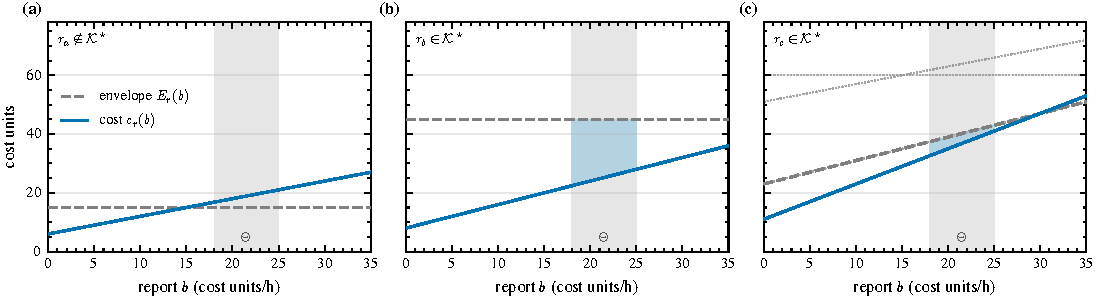
\includegraphics[width=\textwidth]{fig_c1_frontier_intuition.pdf}
\caption{Local margins in Example~\ref{ex:twin}. Solid lines: reported cost
$c_r(b)$; dashed: FD-completion envelope $E_r(b)$ (dotted in (c): its three
affine branches); grey band: report domain $\Theta=[18,25]$. A route belongs
to $\Kstar$ if and only if the envelope lies strictly above its cost
somewhere in $\Theta$ (shaded). Route $r_a$ is deleted only because $\Theta$
excludes reports below 15; with unrestricted reports it would be retained
(Remark~\ref{rem:monotone}).}
\label{fig:frontier-intuition}
\end{figure}

\paragraph{Main result.} The next theorem answers TQ1: deleting every route
outside the frontier is safe.

\begin{theorem}[Safety of the local frontier]
\label{thm:frontier}
Let $\lth<\uth$ and let every pool satisfy Assumption~\ref{ass:nodup}. Then
$\Pi^\star$ is safe: $V(R^{\Pi^\star};b)=V(R;b)$ for every instance and every
$b\in\Theta^N$. Moreover $V_{-k}(R^{\Pi^\star};b)=V_{-k}(R;b)$ for every
driver $k$ and every $b\in\Theta^N$.
\end{theorem}

The difficulty is that a deleted route must be replaced by a route that is
itself \emph{retained}. Its envelope may be attained by a subset route that
is also outside the frontier, which would then also be deleted. The
following lemma shows that a retained substitute always exists.

\begin{lemma}[A retained substitute exists]
\label{lem:substitute}
Let $R_i$ satisfy Assumption~\ref{ass:nodup} and $\lth<\uth$. For every
$r\in R_i\setminus\Kstar_i$ and every $b\in\Theta$ there is
$u\in\Kstar_i\cup\{0_i\}$ with $S_u\subseteq S_r$ and
$c_u(b)+q(S_r\setminus S_u)\le c_r(b)$.
\end{lemma}

\paragraph{Idea of the proof.} Fix $b$ and consider all ways of serving
$S_r$ with $r$ itself or with one subset route plus FD. Among the cheapest of
these, take one whose bundle $T$ is as small as possible. If $T$ is empty,
the idle route $0_i$ is the substitute. Otherwise every smaller alternative is
strictly more expensive at $b$, and these strict inequalities between lines
in the report remain true for reports close to $b$. Among the cheapest routes
with bundle $T$, which have pairwise different slopes $W$ by
Assumption~\ref{ass:nodup}, the one with the smallest slope (or the largest,
if $b=\uth$) becomes strictly cheapest after a small move of the report
inside $\Theta$. At that report its margin is positive, so it belongs to
$\Kstar_i$. The full proof is in Appendix~\ref{app:proofs}.

\begin{proof}[Proof of Theorem~\ref{thm:frontier}]
Fix an instance, a profile $b\in\Theta^N$ and an optimal allocation $\rho$
for the full pools. For every driver $j$ whose route $\rho_j$ is not in
$\Kstar_j\cup\{0_j\}$, Lemma~\ref{lem:substitute} gives
$u_j\in\Kstar_j\cup\{0_j\}$ with $S_{u_j}\subseteq S_{\rho_j}$ and
$c_{u_j}(b_j)+q(S_{\rho_j}\setminus S_{u_j})\le c_{\rho_j}(b_j)$. Replace
$\rho_j$ by $u_j$ and send $S_{\rho_j}\setminus S_{u_j}$ to FD. Bundles only
shrink, so they remain disjoint; every order is still served once; and no
other driver is affected, so all replacements can be made simultaneously.
The resulting allocation uses only pruned pools and costs at most
$V(R;b)$, so $V(R^{\Pi^\star};b)\le V(R;b)$; the reverse inequality holds
because pruned pools are subsets. Removing driver $k$ yields another
instance in which every remaining driver has the same local view, so the
same argument applies to $V_{-k}$.
\end{proof}

\begin{corollary}[VCG outcomes are preserved]
\label{cor:vcg}
Running Algorithms~B and~C on $R^{\Pi^\star}$ is VCG on a bid-independent
range and is therefore truthful and individually rational. At every profile
at which the full problem has a unique optimal allocation, the pruned problem
has the same allocation and every payment~\eqref{eq:payment} coincides with
its full-pool value.
\end{corollary}

\begin{proof}
The first statement is Proposition~\ref{prop:dsic}. Under uniqueness, any
pruned optimum has value $V(R;b)$ by Theorem~\ref{thm:frontier} and is
feasible for the full pools, hence equal to the full optimum; $V$ and every
$V_{-k}$ coincide by Theorem~\ref{thm:frontier}.
\end{proof}

\paragraph{Scope of the result.}

\begin{remark}[What the frontier does not do]
\label{rem:scope}
The theorem guarantees safety, not that the frontier is small. Rules outside
the local class can keep fewer routes. (i) \emph{Non-local rules} that use
the public data of other drivers remain bid-independent, but deciding
exactly which routes they may delete requires reasoning about the other
drivers' winner-determination problem, which is NP-hard for $B\ge 3$ already
at a single report profile: with one driver per 3-set, each owning one route
of cost zero, and $q_o=1$, the optimal value is zero if and only if an exact
cover by 3-sets exists. (ii) \emph{Instance-specific rules}, which only need
to be correct on the instance at hand, can retain far less: on five
experimental instances only 0.4--1.5\% of generated routes are optimal for
any of 1,000 sampled report profiles, whereas the frontier retains 3--23\% of
the pool on the same instances.
\end{remark}

\begin{remark}[Monotonicity]
\label{rem:monotone}
$E_r$ is nondecreasing in every $q_o$, and the maximum of $\mu_r$ over a
larger interval is larger. The frontier therefore grows with the FD tariff
and with the width of $\Theta$: local pruning is strong when FD is cheap and
weak when it is expensive. With $\Theta=[0,\infty)$ the rule remains safe but
retains more routes.
\end{remark}

\begin{remark}[Computation]
\label{rem:computation}
$|D(r)|\le 2^Bf$, where $f$ bounds the number of routes per bundle. Since
$\mu_r$ is concave, membership in $\Kstar_i$ is decided by evaluating $\mu_r$
at the endpoints of $\Theta$ and at the breakpoints of $E_r$, in
$O(|D(r)|\log|D(r)|)$ time; the whole frontier of a driver costs
$O(|R_i|\,2^Bf\log(2^Bf))$. The frontier is a post-processing step: it does
not speed up enumeration, but it shrinks every problem solved by
Algorithms~B and~C. Procedure~\ref{alg:frontier} states the computation.
\end{remark}

\begin{algorithm}[!htbp]
\caption{\textsc{Frontier}$(R_i,q,\Theta)$: the rule $\Pi^\star$ for one driver}
\label{alg:frontier}
\begin{algorithmic}[1]
\Require pool $R_i$ with bundles $S_r$ and coefficients $(K_r,W_r)$; FD prices $q$; $\Theta=[\lth,\uth]$
\Ensure local frontier $\Kstar_i\subseteq R_i$
\State $\Kstar_i\gets\emptyset$
\For{each $r\in R_i$}
  \State $D(r)\gets\{r'\in R_i\cup\{0_i\}\setminus\{r\}:S_{r'}\subseteq S_r\}$
  \State for each $r'\in D(r)$ form the line $g_{r'}(b)=K_{r'}+q(S_r\setminus S_{r'})+b\,W_{r'}$
  \State compute the lower envelope $E_r=\min_{r'\in D(r)}g_{r'}$ on $\Theta$ \Comment{$O(|D(r)|\log|D(r)|)$}
  \State $\mathcal B\gets\{\lth,\uth\}\cup\{\text{breakpoints of }E_r\text{ in }\Theta\}$
  \If{$\max_{b\in\mathcal B}\bigl(E_r(b)-K_r-b\,W_r\bigr)>0$} \Comment{$\mu_r$ is concave}
    \State add $r$ to $\Kstar_i$
  \EndIf
\EndFor
\State \Return $\Kstar_i$
\end{algorithmic}
\end{algorithm}

\begin{remark}[Relation to column dominance and redundancy]
\label{rem:lp}
In the linear relaxation of~\eqref{eq:wdp} let $\pi_o$ be the duals of the
order constraints and $\sigma_i\le 0$ that of driver $i$'s constraint. The FD
columns impose $\pi_o\le q_o$. If $S_{r'}\subseteq S_r$ and
$c_r\ge c_{r'}+q(S_r\setminus S_{r'})$, then, since both routes belong to
driver $i$, the term $\sigma_i$ cancels and
\[
\bar c_r-\bar c_{r'}=c_r-c_{r'}-\pi(S_r\setminus S_{r'})
\ge\sum_{o\in S_r\setminus S_{r'}}(q_o-\pi_o)\ge 0
\]
for every dual vector with $\pi\le q$. The rule $\Pi^\star$ thus deletes a
route when, at each admissible report, a route of the same driver dominates
it in reduced cost over the dual domain restricted by the outside option.
Equivalently, $r$ is redundant in the sense of \citet{sol1994column}, with
the combination consisting of $r'$ and the FD columns of
$S_r\setminus S_{r'}$.
\end{remark}

% ---------------------------------------------------------------------
\subsection{Payment computation}
\label{sec:sd-payments}

Exact payments~\eqref{eq:payment} require one removal solve per winner.
The reference implementation re-solves the base model once per winner with
all variables of that winner fixed to zero (Procedure~\ref{alg:payments}).

\begin{algorithm}[!htbp]
\caption{\textsc{Payments}$(R,b,x^\ast)$: exact Clarke-pivot payments (Algorithm C)}
\label{alg:payments}
\begin{algorithmic}[1]
\Require pools $R$ (fixed before reports), reports $b$, optimal allocation $x^\ast$ with value $V(R;b)$
\Ensure payments $(p_i)_{i\in N}$
\For{each driver $i$}
  \If{$i$ receives no route in $x^\ast$} $p_i\gets 0$; \textbf{continue} \EndIf
  \State fix $x_{ir}=0$ for all $r\in R_i$; re-solve~\eqref{eq:wdp} to optimality with the same tie-breaking
  \State $p_i\gets c_{ir_i^\ast}(b_i)+V_{-i}(R;b)-V(R;b)$
\EndFor
\State \Return $(p_i)_{i\in N}$
\end{algorithmic}
\end{algorithm}

% ---------------------------------------------------------------------
\subsection{Further results planned for the final thesis}
\label{sec:sd-planned}

This proposal establishes the safety of the frontier. Three further
questions from Section~\ref{sec:problem} will be developed, with statements
and proofs, in the final thesis. Preliminary checks for each are already
available.

\subsubsection{Minimality and worst-case size of the frontier (TQ2)}
\label{sec:sd-pol}

The plan is to show that the frontier cannot be improved by any rule of the
same kind: every route in $\Kstar_i$ should be indispensable in some instance
that looks identical from driver $i$'s own data, so that no safe local rule
can delete it. The planned proof adds to driver $i$ cheap single-order
competitors for every order outside the route's bundle. A second planned
result is a family of instances in which a gigworker's frontier contains
$\sum_{k\le B}\binom nk=\Theta(n^B)$ routes, none of which is ever optimal.
Such a result would show that the gap between gigworkers and occasional
drivers is structural. In a synthetic audit, every one of 1,157 frontier
routes was indeed indispensable in the constructed instance, and the planned
worst-case family behaved as predicted for $n=3,5,7,9$.

\subsubsection{Pruning during route generation (TQ3)}
\label{sec:sd-label}

The frontier is computed only after every route has been enumerated. A
\emph{label rule} would apply the same reasoning to partial routes during
enumeration: if dropping an order already picked up, and sending it to FD,
is guaranteed to be cheaper for every completion and every admissible report,
the partial route and all its extensions can be discarded. The direct
transfer of rollback pruning \citep{lozano2016exact} is unsafe here, because
working time is priced and waiting is allowed: a time saving on the known
part of the route can be absorbed by waiting later. A corrected rule with
\emph{junction} and \emph{absorption} terms has been designed and audited.
In an experimental build it left the frontier and every payment unchanged
(maximum difference $5.7\times10^{-14}$) and removed 15--43\% of label
extensions, but in pure Python its bookkeeping made route generation slower
(median time ratio 0.52--0.87). The final thesis will state the rule and
prove that it never changes the frontier.

\subsubsection{Decomposing the payment computation (TQ4)}
\label{sec:sd-decomp}

The \emph{conflict graph} links two drivers whenever some of their routes
share an order; it is built once from the pools, before any report is
read. When the FD price of each order is a fixed constant, the
counterfactual problem of a winner should involve only the connected
component of the graph that contains that winner, so each payment would
require re-solving a smaller problem. This property fails if the fixed fleet
has a shared capacity: removing one driver can then change the allocation in
a component that does not contain that driver. A small counterexample with
two orders and a fleet that can serve only one order has already been
constructed. On the experimental instances, the conflict graph was almost
always connected where the crowd is competitive, so the decomposition is
expected to bring little benefit there. The final thesis will give the
decomposition result with its proof.
% ---------------------------------------------------------------------
\subsection{A small numerical solution}
\label{sec:sd-example}

This section runs the complete procedure by hand on a small instance with
four orders, two gigworkers and two occasional drivers. All numbers are
illustrative; they were chosen so that every step can be checked by hand,
and every value below was recomputed by exhaustive enumeration.

\paragraph{Input.} The bundle cap is $B=2$, the distance coefficient is
$\kappa=0.5$ for every driver, the speed is 20\,km/h, every driver has
capacity 2, and the report domain is $\Theta=[18,25]$.
Table~\ref{tab:ex-input} lists the orders and drivers. The true values of
time are private; the platform never sees them.

\begin{table}[t]
\centering
\caption{Input of the numerical example}
\label{tab:ex-input}
\small
\setlength{\tabcolsep}{4pt}
\begin{tabular}{lccc@{\hspace{0.8cm}}llccc}
\toprule
\multicolumn{4}{c}{Orders} & \multicolumn{5}{c}{Drivers}\\
\cmidrule(r{0.6cm}){1-4}\cmidrule(l){5-9}
Order & Pickup & Delivery & $q_o$ & Driver & Class & Direct trip & Detour & True $\theta_i$\\
\midrule
$o_1$ & $P_1$ & $D_1$ & 15 & $g_1$ & GW & -- & -- & 20\\
$o_2$ & $P_2$ & $D_2$ & 45 & $g_2$ & GW & -- & -- & 24\\
$o_3$ & $P_3$ & $D_3$ & 40 & $c_1$ & OD & 10 km / 30 min & 20 min & 18\\
$o_4$ & $P_4$ & $D_4$ & 50 & $c_2$ & OD & 8 km / 24 min & 18 min & 22\\
\bottomrule
\end{tabular}
\end{table}

\paragraph{Step 1: route generation (Algorithm A).} For the occasional
driver $c_1$ the detour budget of 20 minutes eliminates every bundle that
contains $o_1$ or $o_4$, since a lower bound on their detour (34 and 29
minutes) already exceeds it; only $\{o_2\}$, $\{o_3\}$ and $\{o_2,o_3\}$
remain, out of ten bundles of size at most two. For the gigworker $g_1$ no
such bound exists: order $o_3$ is infeasible because of its time window, and
the pairs $\{o_1,o_4\}$ and $\{o_2,o_4\}$ are infeasible although each of
their orders is feasible on its own, which can only be discovered by
building the sequences. To keep the example small, it uses the nine routes
of Table~\ref{tab:ex-pool}; the routes of $g_1$ serving $\{o_4\}$ and of
$c_1$ serving $\{o_3\}$ alone are left out, and all values below refer to
this pool.

\begin{table}[t]
\centering
\caption{Route pool of the numerical example and reported costs at the true values of time}
\label{tab:ex-pool}
\small
\begin{tabular}{lllccccc}
\toprule
Route & Driver & Bundle & Distance & Time & $K$ & $W$ (h) & $c=K+\theta W$\\
\midrule
$r_1$ & $g_1$ & $\{o_1\}$ & 12 km & 36 min & 6.0 & 0.600 & 18.00\\
$r_2$ & $g_1$ & $\{o_2\}$ & 16 km & 48 min & 8.0 & 0.800 & 24.00\\
$r_3$ & $g_1$ & $\{o_1,o_2\}$ & 22 km & 72 min & 11.0 & 1.200 & 35.00\\
$r_4$ & $g_2$ & $\{o_3\}$ & 10 km & 30 min & 5.0 & 0.500 & 17.00\\
$r_5$ & $g_2$ & $\{o_4\}$ & 14 km & 42 min & 7.0 & 0.700 & 23.80\\
$r_6$ & $g_2$ & $\{o_3,o_4\}$ & 20 km & 60 min & 10.0 & 1.000 & 34.00\\
$r_7$ & $c_1$ & $\{o_2\}$ & 4 km (detour) & 15 min (detour) & 2.0 & 0.250 & 6.50\\
$r_8$ & $c_1$ & $\{o_2,o_3\}$ & 6 km (detour) & 20 min (detour) & 3.0 & 0.333 & 9.00\\
$r_9$ & $c_2$ & $\{o_4\}$ & 3 km (detour) & 15 min (detour) & 1.5 & 0.250 & 7.00\\
\bottomrule
\end{tabular}
\end{table}

\paragraph{Step 2: the local frontier.} For every route, the frontier
compares its cost with the envelope $E_r$ of~\eqref{eq:envelope} at the ends of
$\Theta$ (all envelopes here are linear on $\Theta$, so the endpoints
suffice). Table~\ref{tab:ex-frontier} gives the result. Only $r_1$ is
deleted: serving $o_1$ costs $g_1$ at least $16.80$ at any admissible report,
more than the FD price of 15. Route $r_3$ is kept although $r_1$ is deleted,
because the bundle $\{o_1,o_2\}$ is cheaper than $r_2$ plus FD for $o_1$
(margin 4.80 at $b=18$). This is the twin situation of Example~\ref{ex:twin}.

\begin{table}[t]
\centering
\caption{Local frontier of the numerical example, $\Theta=[18,25]$}
\label{tab:ex-frontier}
\small
\begin{tabular}{llcccccc}
\toprule
Route & $D(r)$ & $E_r(18)$ & $c_r(18)$ & $\mu_r(18)$ & $E_r(25)$ & $c_r(25)$ & In $\Kstar$?\\
\midrule
$r_1$ & $0$ & 15.00 & 16.80 & $-1.80$ & 15.00 & 21.00 & No\\
$r_2$ & $0$ & 45.00 & 22.40 & 22.60 & 45.00 & 28.00 & Yes\\
$r_3$ & $r_1,r_2,0$ & 37.40 & 32.60 & 4.80 & 43.00 & 41.00 & Yes\\
$r_4$ & $0$ & 40.00 & 14.00 & 26.00 & 40.00 & 17.50 & Yes\\
$r_5$ & $0$ & 50.00 & 19.60 & 30.40 & 50.00 & 24.50 & Yes\\
$r_6$ & $r_4,r_5,0$ & 59.60 & 28.00 & 31.60 & 64.50 & 35.00 & Yes\\
$r_7$ & $0$ & 45.00 & 6.50 & 38.50 & 45.00 & 8.25 & Yes\\
$r_8$ & $r_7,0$ & 46.50 & 9.00 & 37.50 & 48.25 & 11.33 & Yes\\
$r_9$ & $0$ & 50.00 & 6.00 & 44.00 & 50.00 & 7.75 & Yes\\
\bottomrule
\end{tabular}
\par\smallskip\footnotesize $0$ denotes the idle route; $E_r(b)$ for $r_3$ is attained by $r_2$ plus FD for $o_1$, and for $r_6$ by $r_5$ plus FD for $o_3$.
\end{table}

\paragraph{Step 3: winner determination (Algorithm B).} With truthful
reports, the optimal allocation gives $r_8=\{o_2,o_3\}$ to $c_1$ and
$r_9=\{o_4\}$ to $c_2$, and sends $o_1$ to FD:
\[
V=9.00+7.00+15=31.00 .
\]
The second-best allocation costs 34.00: it adds $r_1$, so that $g_1$ serves
$o_1$ at a reported cost of 18.00 instead of the FD price of 15. This is the
route deleted by the frontier, and it is used only by a worse allocation.
Both gigworkers lose. The same optimum is obtained on the pruned pool, as
Theorem~\ref{thm:frontier}(a) guarantees.

\paragraph{Step 4: payments (Algorithm C).} Each winner is removed in turn
and the problem re-solved:
\begin{align*}
V_{-c_1}&=c_{r_3}+c_{r_4}+c_{r_9}=35.00+17.00+7.00=59.00,\\
p_{c_1}&=c_{r_8}+V_{-c_1}-V=9.00+59.00-31.00=37.00,\\
V_{-c_2}&=q_{o_1}+c_{r_8}+c_{r_5}=15+9.00+23.80=47.80,\\
p_{c_2}&=c_{r_9}+V_{-c_2}-V=7.00+47.80-31.00=23.80.
\end{align*}
Without $c_1$, gigworker $g_1$ takes the bundle $\{o_1,o_2\}$ and $g_2$ takes
$o_3$; without $c_2$, gigworker $g_2$ takes $o_4$. Table~\ref{tab:ex-money}
summarises the financial outcome. The platform pays 75.80 in total, against
150 if every order were sent to FD; the difference between payments and true
costs, 44.80, is the information rent that buys truthfulness. All values,
including the counterfactuals, are identical on the pruned pool.

\begin{table}[t]
\centering
\caption{Financial outcome of the numerical example}
\label{tab:ex-money}
\small
\begin{tabular}{lccccc}
\toprule
Driver & Route & True cost & $V_{-i}$ & Payment $p_i$ & Utility $p_i-C_i$\\
\midrule
$c_1$ & $r_8$ & 9.00 & 59.00 & 37.00 & 28.00\\
$c_2$ & $r_9$ & 7.00 & 47.80 & 23.80 & 16.80\\
$g_1$, $g_2$ & -- & -- & -- & 0 & 0\\
\midrule
\multicolumn{2}{l}{Optimal value $V$} & \multicolumn{4}{l}{31.00 (routes 16.00, FD 15.00)}\\
\multicolumn{2}{l}{Total platform outlay} & \multicolumn{4}{l}{$37.00+23.80+15=75.80$ (all-FD: 150.00)}\\
\multicolumn{2}{l}{Information rent} & \multicolumn{4}{l}{$28.00+16.80=44.80$}\\
\bottomrule
\end{tabular}
\end{table}

\paragraph{Step 5: checking truthfulness.} Table~\ref{tab:ex-dsic} lets each
driver misreport within $\Theta$. A winner who misreports keeps the same
bundle, her payment does not change, and her utility does not change: the
Clarke-pivot payment depends on her own report only through which bundle she
wins. A loser who underbids to the lower end of $\Theta$ still loses. No
driver gains by misreporting, as Proposition~\ref{prop:dsic} guarantees.

\begin{table}[t]
\centering
\caption{Outcome of unilateral misreports in the numerical example}
\label{tab:ex-dsic}
\small
\begin{tabular}{lcccccc}
\toprule
Driver & True $\theta_i$ & Report $b_i$ & Wins & $V$ & Payment & Utility (true)\\
\midrule
$c_1$ & 18 & 18 (truthful) & $r_8$ & 31.00 & 37.00 & 28.00\\
$c_1$ & 18 & 18.5 & $r_8$ & 31.17 & 37.00 & 28.00\\
$c_1$ & 18 & 25 & $r_8$ & 33.33 & 37.00 & 28.00\\
$c_2$ & 22 & 22 (truthful) & $r_9$ & 31.00 & 23.80 & 16.80\\
$c_2$ & 22 & 18 & $r_9$ & 30.00 & 23.80 & 16.80\\
$c_2$ & 22 & 25 & $r_9$ & 31.75 & 23.80 & 16.80\\
$g_1$ & 20 & 18 & -- & 31.00 & 0 & 0\\
$g_2$ & 24 & 18 & -- & 31.00 & 0 & 0\\
\bottomrule
\end{tabular}
\end{table}

\paragraph{Step 6: payment decomposition.} Driver $g_1$ shares $o_2$ with
$c_1$, $c_1$ shares $o_3$ with $g_2$, and $g_2$ shares $o_4$ with $c_2$. The
conflict graph is a single component, so the planned decomposition of
Section~\ref{sec:sd-decomp} would give no saving here; this mirrors the finding of the computational study that the
graph is almost always connected where the crowd is competitive.

% ---------------------------------------------------------------------
\subsection{Implementation}
\label{sec:sd-impl}

The pipeline is implemented in Python~3.7.7. Table~\ref{tab:modules} maps the
components of Procedure~\ref{alg:mechanism} to the modules of the code base.

\begin{table}[t]
\centering
\caption{Implementation of the components}
\label{tab:modules}
\small
\begin{tabular}{P{3.6cm}P{6.0cm}P{4.6cm}}
\toprule
Component & Module (function) & Remarks\\
\midrule
Instance generator & \texttt{instance\_gen.py} (\texttt{generate\_instance}) & Locked, hashed parameters\\
Algorithm A & \texttt{dp\_labeling.py} (\texttt{build\_route\_pool}) $\to$ \texttt{t6\_dp.py} (\texttt{run\_dp}) & Layers 1 and 2\\
Frontier $\Pi^\star$ & \texttt{kstar\_rule.py} (\texttt{local\_frontier}) & Breakpoints of the lower envelope\\
Label rule (experimental) & \texttt{fdrule\_dp.py}; enumerator \texttt{dp\_fast.py} & Not used in the main runs\\
Algorithms B and C & \texttt{rq1\_wdp.py}, \texttt{rq\_common.py} (\texttt{vcg}) & CPLEX 12.10, one thread, zero gap\\
Conflict graph & \texttt{conflict\_graph.py} & Payment decomposition\\
Test oracle & \texttt{brute\_force.py} (\texttt{brute\_pool\_for\_driver}) & Exhaustive enumeration and WDP\\
\bottomrule
\end{tabular}
\end{table}

\paragraph{Solver settings and tie-breaking.} Algorithms~B and~C call CPLEX
12.10 through its Python interface with one thread and relative and absolute
gap tolerances of zero; any solve not reported as optimal is treated as a
failure and is not used. Tie-breaking is implemented in three steps: the
objective is fixed at its optimal value, the number of orders sent to FD is
minimised, and remaining ties are broken lexicographically by route
identifier. Algorithm~C uses the same pool and the same tie-breaking for
every counterfactual problem.

\paragraph{Bid independence.} Algorithm~A and the frontier take no report
as an argument. A hash of every driver's pool is computed before reports are
read, and a regression test checks that the pool and its hash are unchanged
when the reports change.

\paragraph{Verification.} Before any main run, every component was checked
against the independent oracle on instances with $n\in\{3,\dots,6\}$, two
time-window widths, three seeds and four drivers: 360 preliminary checks and
1,035 checks for the later research questions, all passed with deviations
below $10^{-6}$. The theoretical results were additionally audited with a
reference implementation that shares no code with the production one
(Table~\ref{tab:audit1}). It enumerates every precedence-feasible sequence,
computes the frontier analytically, and solves every winner-determination
problem exactly with the HiGHS solver on synthetic instances with $n=8$
orders, two gigworkers and two occasional drivers, $B=3$ and nine seeds.
Deliberate mutations (for example removing the FD term from the envelope)
were detected.

\begin{table}[t]
\centering
\caption{Synthetic audit of the local pruning frontier}
\label{tab:audit1}
\small
\begin{tabular}{P{10.2cm}P{4.0cm}}
\toprule
Check & Result\\
\midrule
Routes after Pareto filtering / retained by $\Pi^\star$ & 2,985 / 1,157 (38.8\%)\\
Max.\ $|V(R^{\Pi^\star})-V(R)|$ over base and removal solves & $5.7\times10^{-14}$\\
Max.\ payment difference (1,737 payments) & $5.7\times10^{-14}$\\
Routes optimal for some of 400 report profiles (three seeds) & 1.9--3.8\% of pool, all in $\Kstar$\\
Frontier routes deleted by a per-driver hull across bundles & 1,144 / 1,157\\
Mutation: FD term removed from $E_r$ & Detected\\
\bottomrule
\end{tabular}
\end{table}

% ---------------------------------------------------------------------
\subsection{Investigation of alternative solutions and the improved solution}
\label{sec:sd-alternatives}

The final design is the result of an iterative development in which each
candidate was tested against brute force and either rejected or improved.
Table~\ref{tab:history} summarises the development path.

\begin{table}[t]
\centering
\caption{Development path of the solution}
\label{tab:history}
\small
\begin{tabular}{P{0.8cm}P{4.0cm}P{5.0cm}P{3.6cm}}
\toprule
Step & Candidate & Finding & Decision\\
\midrule
1 & Level-wise insertion & Complete (0 mismatches, 1,152 instances); sequence count explodes under wide windows & Keep as baseline; needs compression\\
2 & Pareto dominance between sequences & 31.26\% of gigworker bundles lose sequences & Rejected\\
3 & Lookahead-profile dominance & Sound at depth 1; 66.5--72.4\% violations at depth $\ge 2$ & Rejected for generation\\
4 & Self-survival bound & Sound; prunes 0\% under wide windows & Rejected (no effect)\\
5 & Forward label-setting, exact key & 0 violations, including adversarial 2D cases; 5--10$\times$ faster & \textbf{Adopted as Algorithm A}\\
6 & Per-driver hull across bundles & Deletes routes that some instance needs (Example~\ref{ex:twin}) & Rejected\\
7 & Local FD-completion frontier & Safe (Theorem~\ref{thm:frontier}) & \textbf{Adopted as $\Pi^\star$}\\
8 & Rollback pruning transferred directly & Unsafe when waiting is priced & Corrected\\
9 & Label rule with junction and absorption terms & Frontier unchanged in audit; slower in pure Python & Planned (Section~\ref{sec:sd-label})\\
10 & Component decomposition of payments & Exact under separability; fails with shared FD capacity & Planned (Section~\ref{sec:sd-decomp})\\
\bottomrule
\end{tabular}
\end{table}

The improvement from step~1 to step~5 is in completeness and speed: the
label-setting algorithm is provably complete and 5--10 times faster than the
level-wise baseline. The improvement from step~6 to step~7 is in safety:
the per-driver hull is strong but wrong, whereas the frontier is exact for
every admissible report (Theorem~\ref{thm:frontier}). Whether any other
local rule can do better is the subject of the minimality result planned in
Section~\ref{sec:sd-pol}.

% ---------------------------------------------------------------------
\subsection{Comparison of alternative solutions under feasibility constraints and standards}
\label{sec:sd-compare}

\paragraph{Economic feasibility.} On the numerical example,
Table~\ref{tab:ex-alt} compares the selected design with alternative
designs. Using both crowd classes is as good as the better single class here
(both 31.00), and much better than gigworkers alone (69.00). Allowing bundles
lowers the cost from 45.50 (single-order routes) to 31.00, a 31.9\%
reduction. A posted price of $0.8\,q_o$ attracts a cover of all orders, but
since the platform cannot see costs, its payout (120.00) is higher than the
VCG outlay (75.80) and the selected routes have a true cost of at least
59.00. This small example is illustrative only: in the computational study
the optimised posted price paid less than VCG on average but lost about 4\%
efficiency, and the value of joint bidding and bundling depended on whether
the crowd could compete with the fixed fleet (Chapter~5).

\begin{table}[t]
\centering
\caption{Alternative designs on the numerical example (true values of time)}
\label{tab:ex-alt}
\small
\setlength{\tabcolsep}{4pt}
\begin{tabular}{P{4.4cm}P{1.9cm}P{1.9cm}P{2.0cm}P{3.6cm}}
\toprule
Design & True system cost & Platform outlay & Truthful? & Selected routes\\
\midrule
All orders to FD & 150.00 & 150.00 & -- & none\\
Gigworkers only (VCG) & 69.00 & -- & Yes & $r_3$, $r_6$\\
Occasional drivers only (VCG) & 31.00 & -- & Yes & $r_8$, $r_9$\\
Single-order routes only (VCG) & 45.50 & -- & Yes & $r_4$, $r_7$, $r_9$\\
Posted price $0.8\,q_o$ & $\ge 59.00$ & 120.00 & Accept or decline only & e.g.\ $r_3$, $r_4$, $r_9$\\
\textbf{Joint bidding, bundles, VCG (selected)} & \textbf{31.00} & \textbf{75.80} & \textbf{Yes} & $r_8$, $r_9$, FD for $o_1$\\
\bottomrule
\end{tabular}
\par\smallskip\footnotesize Outlay is reported only where a payment rule is specified for the design. Under the posted price every cover of all orders has the same payout, so the true cost depends on tie-breaking.
\end{table}

\paragraph{Environmental aspects.} The mechanism influences emissions
through the distance driven. Bundling lets one driver serve several orders on
one route, and occasional drivers are charged only for their detour, so
orders that lie along their trips are served with little extra driving. In
the computational study, larger bundles reduced the share of orders sent to
the fixed fleet from 0.897 (single-order routes) to 0.731 with $B=3$. The
model does not price emissions; the ISO~14083:2023 standard for quantifying
greenhouse-gas emissions of transport chains would provide a consistent basis
for converting the distances of selected routes into emissions in an
extension.

\paragraph{Social aspects.} For drivers, the mechanism makes truthful
reporting a dominant strategy and guarantees nonnegative utility to
winners, so drivers with little experience in bidding are not disadvantaged
by others' strategic skill. Publishing a hash of the route pool before
bidding lets drivers verify that the allocation range was not changed after
the bids were seen. The pre-auction certificate avoids inviting drivers who
cannot win at any admissible report. The mechanism does not address
minimum earnings, working-hour limits or fairness across drivers, which
platforms must handle under applicable labour regulation.

\paragraph{Data and information security.} The mechanism collects one
number per driver and uses location and trip data of occasional drivers.
Such data are personal data; a deployment in Vietnam would have to comply
with the Law on Personal Data Protection (Law No.~91/2025/QH15, in force
since 1 January 2026) and its guiding Decree No.~356/2025/ND-CP, which
replaced Decree No.~13/2023/ND-CP, and an information-security management
system such as ISO/IEC~27001 would govern their storage and access.
Standards such as OSHA, HACCP or TCVN product standards do not apply directly
to a procurement algorithm.

\paragraph{Summary.} Among the alternatives, the selected design is the only
one that satisfies all correctness requirements R1--R7 simultaneously:
exact VCG on a bid-independent pool reduced to the local frontier. Its costs
are a payout premium over true costs (the information rent) and the work of
enumerating the pool, which for gigworkers grows quickly with the number of
orders. Chapter~5 quantifies both on
the full experimental grid.

% \input{chapters/ch5_result_analysis}   % TODO: Chapter 5
% \input{chapters/ch6_conclusions}       % TODO: Chapter 6

% =====================================================================
% References and appendices
% =====================================================================
%% =====================================================================
%% References -- APA style, alphabetical (IEM-IU guideline, Appendix K).
%% Entries marked "% VERIFY" were flagged in Paper.tex: confirm authors,
%% title, venue, volume, issue and pages against the publisher record.
%% Entries added for the thesis (2021-2026) were checked online on
%% 2026-10-01 (title, authors, venue, volume, pages, DOI where given).
%% =====================================================================
\clearpage
\phantomsection
\addcontentsline{toc}{chapter}{References}
\renewcommand{\bibname}{References}
\begin{singlespace}
\begin{thebibliography}{99}
\setlength{\itemsep}{4pt}

\bibitem[Aggarwal and Hartline(2006)]{aggarwal2006knapsack}
Aggarwal, G., \& Hartline, J. D. (2006). Knapsack auctions. In
\emph{Proceedings of the 17th Annual ACM-SIAM Symposium on Discrete
Algorithms} (pp.~1083--1092). SIAM. % VERIFY

\bibitem[Alnaggar et~al.(2021)]{alnaggar2021crowdsourced}
Alnaggar, A., Gzara, F., \& Bookbinder, J. H. (2021). Crowdsourced delivery:
A review of platforms and academic literature. \emph{Omega}, \emph{98},
102139. https://doi.org/10.1016/j.omega.2019.102139

\bibitem[Archetti et~al.(2016)]{archetti2016vrpod}
Archetti, C., Savelsbergh, M., \& Speranza, M. G. (2016). The vehicle
routing problem with occasional drivers. \emph{European Journal of
Operational Research}, \emph{254}(2), 472--480.

\bibitem[Ausseil et~al.(2022)]{ausseil2022supplier}
Ausseil, R., Pazour, J. A., \& Ulmer, M. W. (2022). Supplier menus for
dynamic matching in peer-to-peer transportation platforms.
\emph{Transportation Science}, \emph{56}(5), 1304--1326.

\bibitem[Beasley(1987)]{beasley1987algorithm}
Beasley, J. E. (1987). An algorithm for set covering problem.
\emph{European Journal of Operational Research}, \emph{31}(1), 85--93.
% VERIFY: dominance rule read in original

\bibitem[Ben Amor et~al.(2006)]{benamor2006dual}
Ben Amor, H., Desrosiers, J., \& Val{\'e}rio de Carvalho, J. M. (2006).
Dual-optimal inequalities for stabilized column generation.
\emph{Operations Research}, \emph{54}(3), 454--463.

\bibitem[Bleischwitz and Kliewer(2005)]{bleischwitz2005accelerating}
Bleischwitz, Y., \& Kliewer, G. (2005). Accelerating Vickrey payment
computation in combinatorial auctions for an airline alliance. In
\emph{Experimental and Efficient Algorithms (WEA 2005)}, Lecture Notes in
Computer Science 3503. Springer. % VERIFY: page range

\bibitem[Boysen et~al.(2021)]{boysen2021lastmile}
Boysen, N., Fedtke, S., \& Schwerdfeger, S. (2021). Last-mile delivery
concepts: A survey from an operational research perspective. \emph{OR
Spectrum}, \emph{43}, 1--58. https://doi.org/10.1007/s00291-020-00607-8

\bibitem[B{\"u}nz et~al.(2015)]{bunz2015faster}
B{\"u}nz, B., Seuken, S., \& Lubin, B. (2015). A faster core constraint
generation algorithm for combinatorial auctions. In \emph{Proceedings of
the 29th AAAI Conference on Artificial Intelligence} (pp.~827--834).

\bibitem[Chen et~al.(2023)]{chen2023truthful}
Chen et~al. (2023). Truthful combinatorial reverse auction for
occasional-courier crowdsourced delivery. \emph{IEEE Internet of Things
Journal}. % VERIFY: full author list, exact title, volume, issue, pages

\bibitem[Dumas et~al.(1991)]{dumas1991pickup}
Dumas, Y., Desrosiers, J., \& Soumis, F. (1991). The pickup and delivery
problem with time windows. \emph{European Journal of Operational Research},
\emph{54}(1), 7--22.

\bibitem[Ehrgott(2005)]{ehrgott2005multicriteria}
Ehrgott, M. (2005). \emph{Multicriteria optimization} (2nd ed.). Springer.

\bibitem[Feillet et~al.(2004)]{feillet2004exact}
Feillet, D., Dejax, P., Gendreau, M., \& Gueguen, C. (2004). An exact
algorithm for the elementary shortest path problem with resource
constraints: Application to some vehicle routing problems.
\emph{Networks}, \emph{44}(3), 216--229. % VERIFY

\bibitem[Gschwind et~al.(2018)]{gschwind2018bidirectional}
Gschwind, T., Irnich, S., Rothenb{\"a}cher, A.-K., \& Tilk, C. (2018).
Bidirectional labeling in column-generation algorithms for
pickup-and-delivery problems. \emph{European Journal of Operational
Research}, \emph{266}(2), 521--530.

\bibitem[Hershberger and Suri(2001)]{hershberger2001vickrey}
Hershberger, J., \& Suri, S. (2001). Vickrey prices and shortest paths: What
is an edge worth? In \emph{Proceedings of the 42nd IEEE Symposium on
Foundations of Computer Science} (pp.~252--259).

\bibitem[Kempe et~al.(2010)]{kempe2010frugal}
Kempe, D., Salek, M., \& Moore, C. (2010). Frugal and truthful auctions for
vertex covers, flows, and cuts. In \emph{Proceedings of the 51st IEEE
Symposium on Foundations of Computer Science} (pp.~745--754). % VERIFY pages

\bibitem[Li and Zhang(2026)]{li2026auction}
Li, D., \& Zhang, F. (2026). Auction mechanism design for order allocation
and payment in a crowdshipping system. \emph{Transportation Science},
articles in advance. https://doi.org/10.1287/trsc.2025.0089

\bibitem[Lozano et~al.(2016)]{lozano2016exact}
Lozano, L., Duque, D., \& Medaglia, A. L. (2016). An exact algorithm for the
elementary shortest path problem with resource constraints.
\emph{Transportation Science}, \emph{50}(1), 348--357.
https://doi.org/10.1287/trsc.2014.0582 % VERIFY volume/pages

\bibitem[L{\"u}bbecke and Desrosiers(2005)]{lubbecke2005selected}
L{\"u}bbecke, M. E., \& Desrosiers, J. (2005). Selected topics in column
generation. \emph{Operations Research}, \emph{53}(6), 1007--1023.

\bibitem[Luy et~al.(2024)]{luy2024workforce}
Luy, J., Hiermann, G., \& Schiffer, M. (2024). Strategic workforce planning
in crowdsourced delivery with hybrid driver fleets. \emph{Production and
Operations Management}, \emph{33}(11), 2177--2200.

\bibitem[Mancini and Gansterer(2022)]{mancini2022bundle}
Mancini, S., \& Gansterer, M. (2022). Bundle generation for last-mile
delivery with occasional drivers. \emph{Omega}, \emph{108}.
% VERIFY: article number

\bibitem[Mancini and Gansterer(2024)]{mancini2024bundle}
Mancini, S., \& Gansterer, M. (2024). Bundle generation for the vehicle
routing problem with occasional drivers and time windows. \emph{Flexible
Services and Manufacturing Journal}.
https://doi.org/10.1007/s10696-023-09529-3 % VERIFY: volume and pages

\bibitem[Mohri et~al.(2023)]{mohri2023crowdshipping}
Mohri, S. S., Ghaderi, H., Nassir, N., \& Thompson, R. G. (2023).
Crowdshipping for sustainable urban logistics: A systematic review of the
literature. \emph{Transportation Research Part E: Logistics and
Transportation Review}, \emph{178}, 103289.
https://doi.org/10.1016/j.tre.2023.103289

\bibitem[Mousavi et~al.(2022)]{mousavi2022stochastic}
Mousavi, K., Bodur, M., \& Roorda, M. J. (2022). Stochastic last-mile
delivery with crowd-shipping and mobile depots. \emph{Transportation
Science}, \emph{56}(3), 612--630. https://doi.org/10.1287/trsc.2021.1088

\bibitem[M{\"u}ller(1998)]{muller1998solving}
M{\"u}ller, T. (1998). Solving set partitioning problems with constraint
programming. In \emph{Proceedings of the 6th International Conference on
the Practical Application of Prolog and the 4th International Conference
on the Practical Application of Constraint Technology (PAPPACT98)}
(pp.~313--332). % VERIFY venue

\bibitem[Nisan(2007)]{nisan2007agt}
Nisan, N. (2007). Introduction to mechanism design (for computer
scientists). In N. Nisan, T. Roughgarden, {\'E}. Tardos, \& V. V. Vazirani
(Eds.), \emph{Algorithmic game theory} (pp.~209--242). Cambridge University
Press. % VERIFY pages

\bibitem[Nisan and Ronen(2000)]{nisan2000computationally}
Nisan, N., \& Ronen, A. (2000). Computationally feasible VCG mechanisms. In
\emph{Proceedings of the 2nd ACM Conference on Electronic Commerce}
(pp.~242--252).

\bibitem[Nisan and Ronen(2007)]{nisan2007computationally}
Nisan, N., \& Ronen, A. (2007). Computationally feasible VCG mechanisms.
\emph{Journal of Artificial Intelligence Research}, \emph{29}, 19--47.
% VERIFY pages

\bibitem[Oyama and Akamatsu(2025)]{oyama2025market}
Oyama, Y., \& Akamatsu, T. (2025). Market-based matching with task bundling
for crowdsourced delivery. \emph{Transportation Research Part C: Emerging
Technologies}, \emph{174}, 105110. % VERIFY title

\bibitem[Pereira and Averbakh(2013)]{pereira2013robust}
Pereira, J., \& Averbakh, I. (2013). The robust set covering problem with
interval data. \emph{Annals of Operations Research}.
% VERIFY: volume, pages, year

\bibitem[Sandholm et~al.(2005)]{sandholm2005cabob}
Sandholm, T., Suri, S., Gilpin, A., \& Levine, D. (2005). CABOB: A fast
optimal algorithm for winner determination in combinatorial auctions.
\emph{Management Science}, \emph{51}(3), 374--390.

\bibitem[Savelsbergh and Ulmer(2022)]{savelsbergh2022challenges}
Savelsbergh, M., \& Ulmer, M. W. (2022). Challenges and opportunities in
crowdsourced delivery planning and operations. \emph{4OR}, \emph{20}(1),
1--21.

\bibitem[Savelsbergh and Ulmer(2024)]{savelsbergh2024update}
Savelsbergh, M., \& Ulmer, M. W. (2024). Challenges and opportunities in
crowdsourced delivery planning and operations---an update. \emph{Annals of
Operations Research}, \emph{343}(2), 639--661.
https://doi.org/10.1007/s10479-024-06249-1

\bibitem[Sol(1994)]{sol1994column}
Sol, M. (1994). \emph{Column generation techniques for pickup and delivery
problems} [Doctoral dissertation, Eindhoven University of Technology].
% VERIFY: read the thesis itself; currently cited via Lubbecke & Desrosiers (2005)

\bibitem[Torres et~al.(2022a)]{torres2022crowdshipping}
Torres, F., Gendreau, M., \& Rei, W. (2022a). Crowdshipping: An open VRP
variant with stochastic destinations. \emph{Transportation Research Part C:
Emerging Technologies}, \emph{140}, 103677.

\bibitem[Torres et~al.(2022b)]{torres2022stochastic}
Torres, F., Gendreau, M., \& Rei, W. (2022b). Vehicle routing with
stochastic supply of crowd vehicles and time windows. \emph{Transportation
Science}, \emph{56}(3), 631--653. https://doi.org/10.1287/trsc.2021.1101

\bibitem[Triki(2021)]{triki2021combinatorial}
Triki, C. (2021). Combinatorial procurement auction for the crowd-shipping
problem with occasional drivers. \emph{Journal of Cleaner Production}.
% VERIFY: exact title, volume, article number

\bibitem[Val{\'e}rio de Carvalho(2005)]{valerio2005extra}
Val{\'e}rio de Carvalho, J. M. (2005). Using extra dual cuts to accelerate
column generation. \emph{INFORMS Journal on Computing}, \emph{17}(2),
175--182.

\bibitem[Vanderbeck(1994)]{vanderbeck1994thesis}
Vanderbeck, F. (1994). \emph{Decomposition and column generation for
integer programs} [Doctoral dissertation, Universit{\'e} catholique de
Louvain]. % VERIFY: read the thesis itself; currently cited via Lubbecke & Desrosiers (2005)

\bibitem[Wilkens and Sivan(2012)]{wilkens2012single}
Wilkens, C. A., \& Sivan, B. (2012). Single-call mechanisms. In
\emph{Proceedings of the 13th ACM Conference on Electronic Commerce}
(pp.~946--963). % VERIFY: venue and pages (arXiv:1011.6134)

\bibitem[Xu et~al.(2026)]{xu2026incentive}
Xu, R., Wang, Y., Liu, C., Huang, X., \& Zhang, F. (2026).
Incentive-compatible auction mechanisms for crowdshipping.
\emph{Transportation Research Part E: Logistics and Transportation Review}.
% VERIFY: authors, title, volume

\bibitem[Zhou et~al.(2026)]{zhou2026service}
Zhou, B., Zhang, Y., Baldacci, R., \& Tang, J. (2026). The service-centric
vehicle routing problem with crowdshipping. \emph{European Journal of
Operational Research}, \emph{331}(2), 495--519.
https://doi.org/10.1016/j.ejor.2025.10.012

\bibitem[Zou and Kafle(2022)]{zou2022mechanisms}
Zou, B., \& Kafle, N. (2022). Designing mechanisms for crowdsourced urban
parcel delivery. \emph{Transportation Letters}, \emph{15}(8), 992--1010.
% VERIFY year (vol. 15 may be 2023)

\end{thebibliography}
\end{singlespace}


\appendix
\titleformat{\chapter}[block]
  {\centering\bfseries\fontsize{14}{18}\selectfont}
  {Appendix \thechapter}{0.6em}{}
\addtocontents{toc}{\protect\renewcommand{\protect\cftchappresnum}{Appendix }%
  \protect\renewcommand{\protect\cftchapaftersnum}{}}
% =====================================================================
\chapter{PROOF OF THE SUBSTITUTE LEMMA}
\label{app:proofs}
% =====================================================================

This appendix proves Lemma~\ref{lem:substitute}, on which the safety of the
local frontier (Theorem~\ref{thm:frontier}) rests: for every route $r$
outside the frontier and every admissible report $b$, there is a substitute
$u$ in the frontier (or the idle route) with $S_u\subseteq S_r$ and
$c_u(b)+q(S_r\setminus S_u)\le c_r(b)$.

\begin{proof}
Fix $r\notin\Kstar_i$ and $b\in\Theta$. On $\bar D=D(r)\cup\{r\}$ define
$\Phi(\rho)=c_\rho(b)+q(S_r\setminus S_\rho)$, the cost of serving $S_r$ with
route $\rho$ and sending the rest to FD. Since $\mu_r(b)\le 0$,
$m:=\min_{\bar D}\Phi\le\Phi(r)=c_r(b)$. Let $M=\arg\min_{\bar D}\Phi$ and
$k=\min_{\rho\in M}|S_\rho|$, the smallest bundle among the cheapest options.

\emph{Case $k=0$.} Then $0_i\in M$ and $u=0_i$ satisfies
$c_u(b)+q(S_r)=m\le c_r(b)$.

\emph{Case $k\ge 1$.} Fix $\rho_0\in M$ with $|S_{\rho_0}|=k$, let
$T=S_{\rho_0}$ and $M_T=\{\rho\in R_i:S_\rho=T,\;c_\rho(b)=c_{\rho_0}(b)\}$;
every $\rho\in M_T$ has $\Phi(\rho)=m$.

\emph{Claim.} For every $\rho\in M_T$ and every $\rho''\in D(\rho)\setminus M_T$,
$c_{\rho''}(b)+q(T\setminus S_{\rho''})>c_\rho(b)$.
If $S_{\rho''}\subsetneq T$, then $\rho''\in\bar D$ and $|S_{\rho''}|<k$, so
$\rho''\notin M$ and $\Phi(\rho'')>m=\Phi(\rho)$; since
$S_r\setminus S_{\rho''}=(T\setminus S_{\rho''})\cup(S_r\setminus T)$
disjointly, $\Phi(\rho'')-\Phi(\rho)=c_{\rho''}(b)+q(T\setminus S_{\rho''})-c_\rho(b)>0$.
If $S_{\rho''}=T$ and $\rho''\notin M_T$, then $\Phi(\rho'')\ge m$ gives
$c_{\rho''}(b)\ge c_\rho(b)$, and equality would place $\rho''$ in $M_T$.

The claim consists of finitely many strict inequalities between affine
functions of $b$, so there is $\eta>0$ such that they hold for every
$b'\in\Theta$ with $|b'-b|<\eta$. All routes of $M_T$ have bundle $T$ and the
same cost at $b$; by Assumption~\ref{ass:nodup} their slopes $W$ are
pairwise distinct. If $b<\uth$, let $u=\arg\min_{\rho\in M_T}W_\rho$ and choose
$b'\in(b,\min\{b+\eta,\uth\})$: then $c_u(b')<c_\rho(b')$ for all
$\rho\in M_T\setminus\{u\}$, and by the claim at $b'$,
$c_u(b')<c_{\rho''}(b')+q(T\setminus S_{\rho''})$ for all other
$\rho''\in D(u)$. Hence $\mu_u(b')>0$ and $u\in\Kstar_i$. If $b=\uth$, take
$u=\arg\max_{\rho\in M_T}W_\rho$ and $b'<b$ close to $b$; the same argument
applies. In both cases $u\ne r$, since otherwise $\mu_r(b')>0$ would
contradict $r\notin\Kstar_i$. Moreover $S_u=T\subseteq S_r$ and
$c_u(b)+q(S_r\setminus T)=m\le c_r(b)$.
\end{proof}


\end{document}
